% !Mode:: "TeX:UTF-8"
% !TEX program  = xelatex
\documentclass[a4paper]{article}
\usepackage{amsmath}
\usepackage{amssymb}
\usepackage{ctex}
\usepackage{graphicx}
\usepackage[european]{circuitikz}
\usepackage{multirow}
\usepackage{geometry}
\geometry{a4paper, top=2.54cm, bottom=2.54cm, left=2.54cm, right=2.54cm}
\title{波形发生及整形电路实验报告}
\author{王凯灵 521030910356}
\date{2022年11月17日}
\begin{document}
	\maketitle
	\section{实验目的}
	在熟悉集成放大器的电路结构, UA741芯片中的集成运算放大器功能及其引脚连接方法的基础上, 使用UA741芯片中的集成运算放大器实现波形发生及整形电路, 以及使用555定时器芯片设计实现施密特触发器电路. 
	
	\section{实验原理和仪器}
	实验的主要仪器有: 导线若干, DC电源, 通用示波器, 波形发生器, 万用表和JDEE-AD2II 实验箱, 上有电阻电容等电路元件和芯片若干. 
	
	实验使用UA741芯片和555定时器芯片. 其中, UA741芯片介绍已给出, 555定时器芯片内部逻辑电路和引脚示意图如图所示. 
	
	\begin{figure}[h]
		\centering
		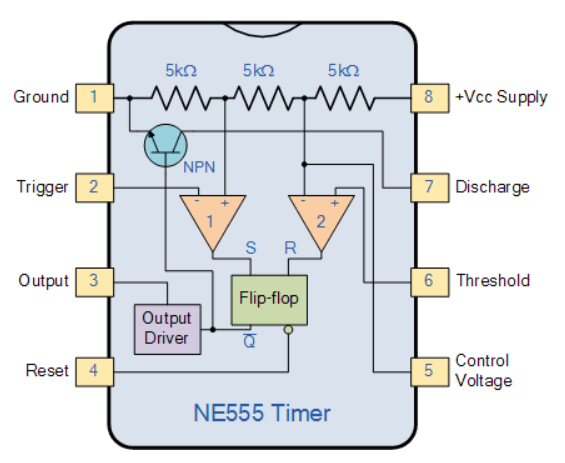
\includegraphics[width=0.3\linewidth]{555定时器}
		\caption{555定时器}
	\end{figure}	
	
	对于UA741芯片, 7端接入 +12V Vcc 直流电源, 4 接入 -12V -Vcc 直流电源. 2为反相输入端, 3为同相输入端, 6为输出. 1和5为偏置(调零端), 8空脚, 通常悬空. 
	
	对于555定时器芯片, 1端接地, 8端接5V Vcc直流供电. 2端为触发端, 4端为复位端. 5端控制端控制芯片阈值电压, 6端用于判断阈值, 7端用于电容放电. 3端为输出端.	
	
	纯滤波电路没有涉及芯片使用. 其电路结构如图.
	
	\begin{figure}[h]
		\centering
		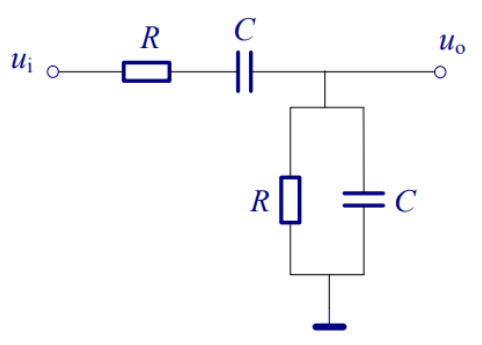
\includegraphics[width=0.3\linewidth]{滤波电路}
		\caption{滤波电路}
	\end{figure}

	考察其输入输出的频率关系, 作频域电路图得
	$$
	\frac{U_o(s)}{U_i(s)}=\frac{R}{R^2 C s+3 R+\frac{1}{c s}}
	$$
	当图中两电阻值相等, 两电容值相等, 中心频率
	$$
	f_0=\frac{1}{2 \pi R C}
	$$
	据此可以设计实验所需电路. 其余波形发生及整形电路也可以使用频域电路图的方法分析. 
	
	\section{实验过程与结果}
	使用DC电源产生串联的双12V直流电源为UA741芯片供电, 使用5V直流电源给555芯片供电. 
	
	\subsection{二阶无源带通滤波器}
	如原理中所述电路连接. 连接实物图如图所示. 
	
	\begin{figure}[h]
		\begin{minipage}[t]{0.5\linewidth}
			\centering
			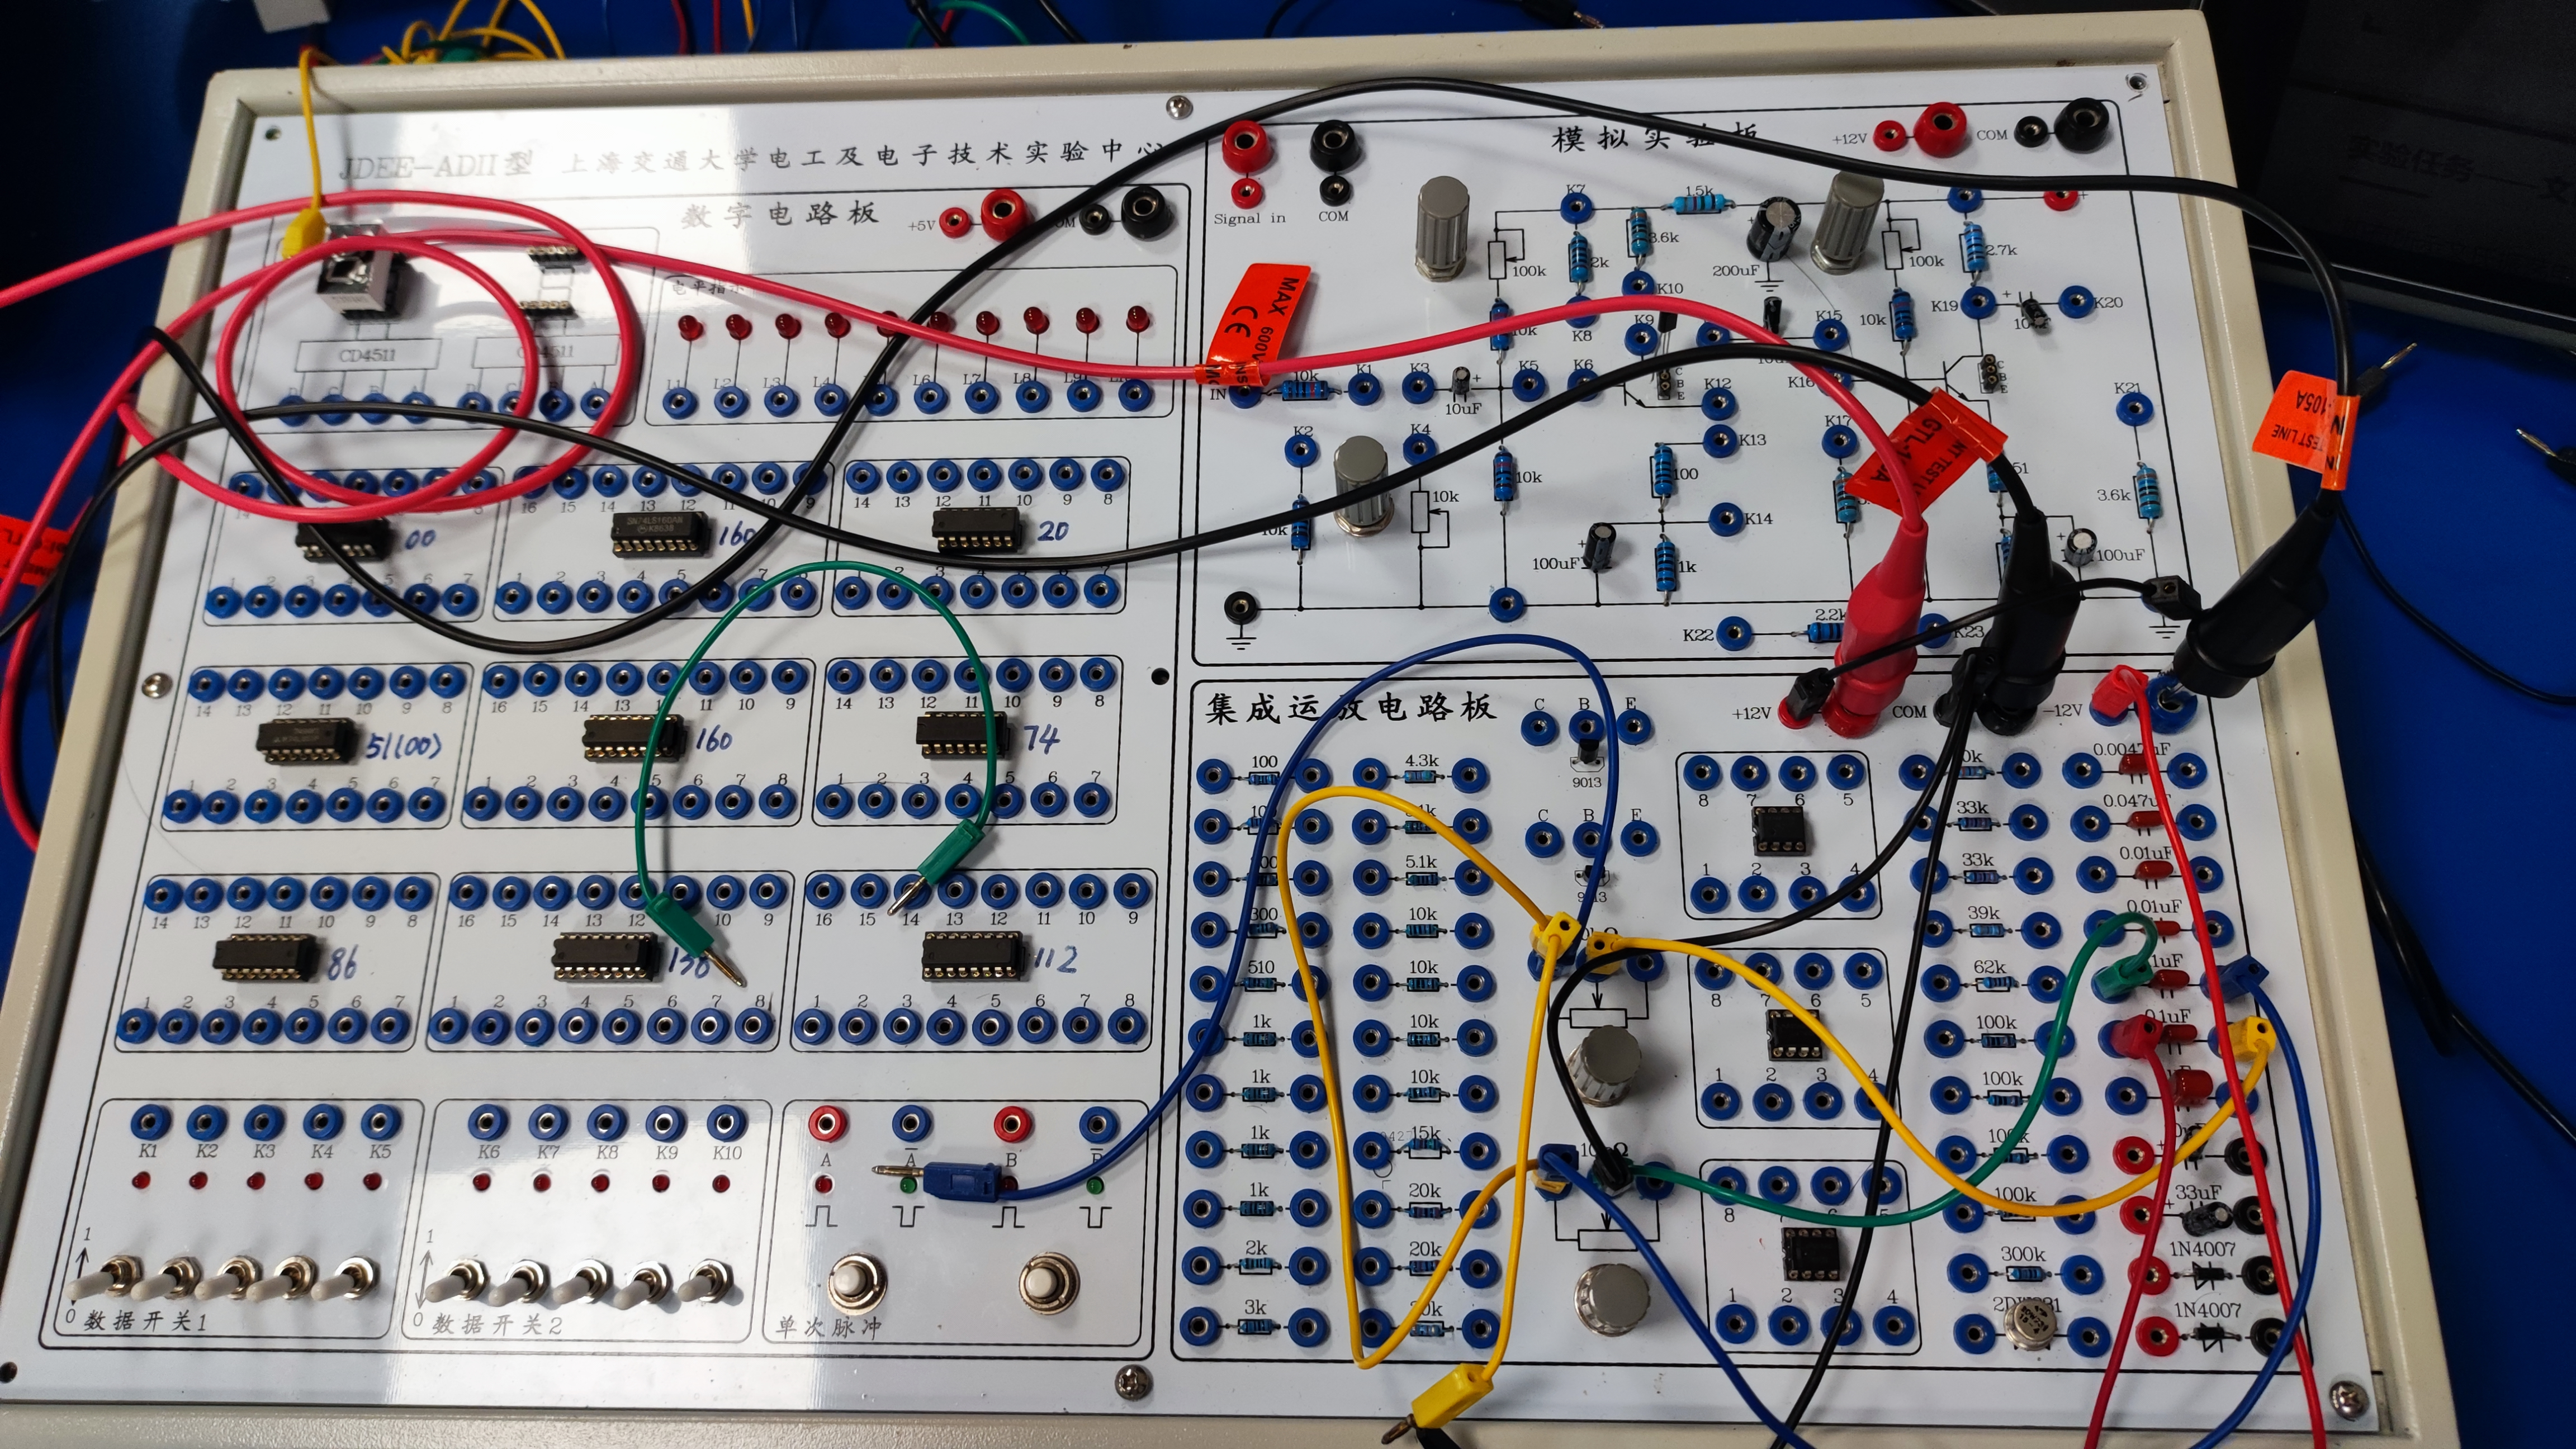
\includegraphics[width=0.9\linewidth]{../图片/滤波器}
			\caption{滤波器实物图}
		\end{minipage}
		\begin{minipage}[t]{0.5\linewidth}
			\centering
			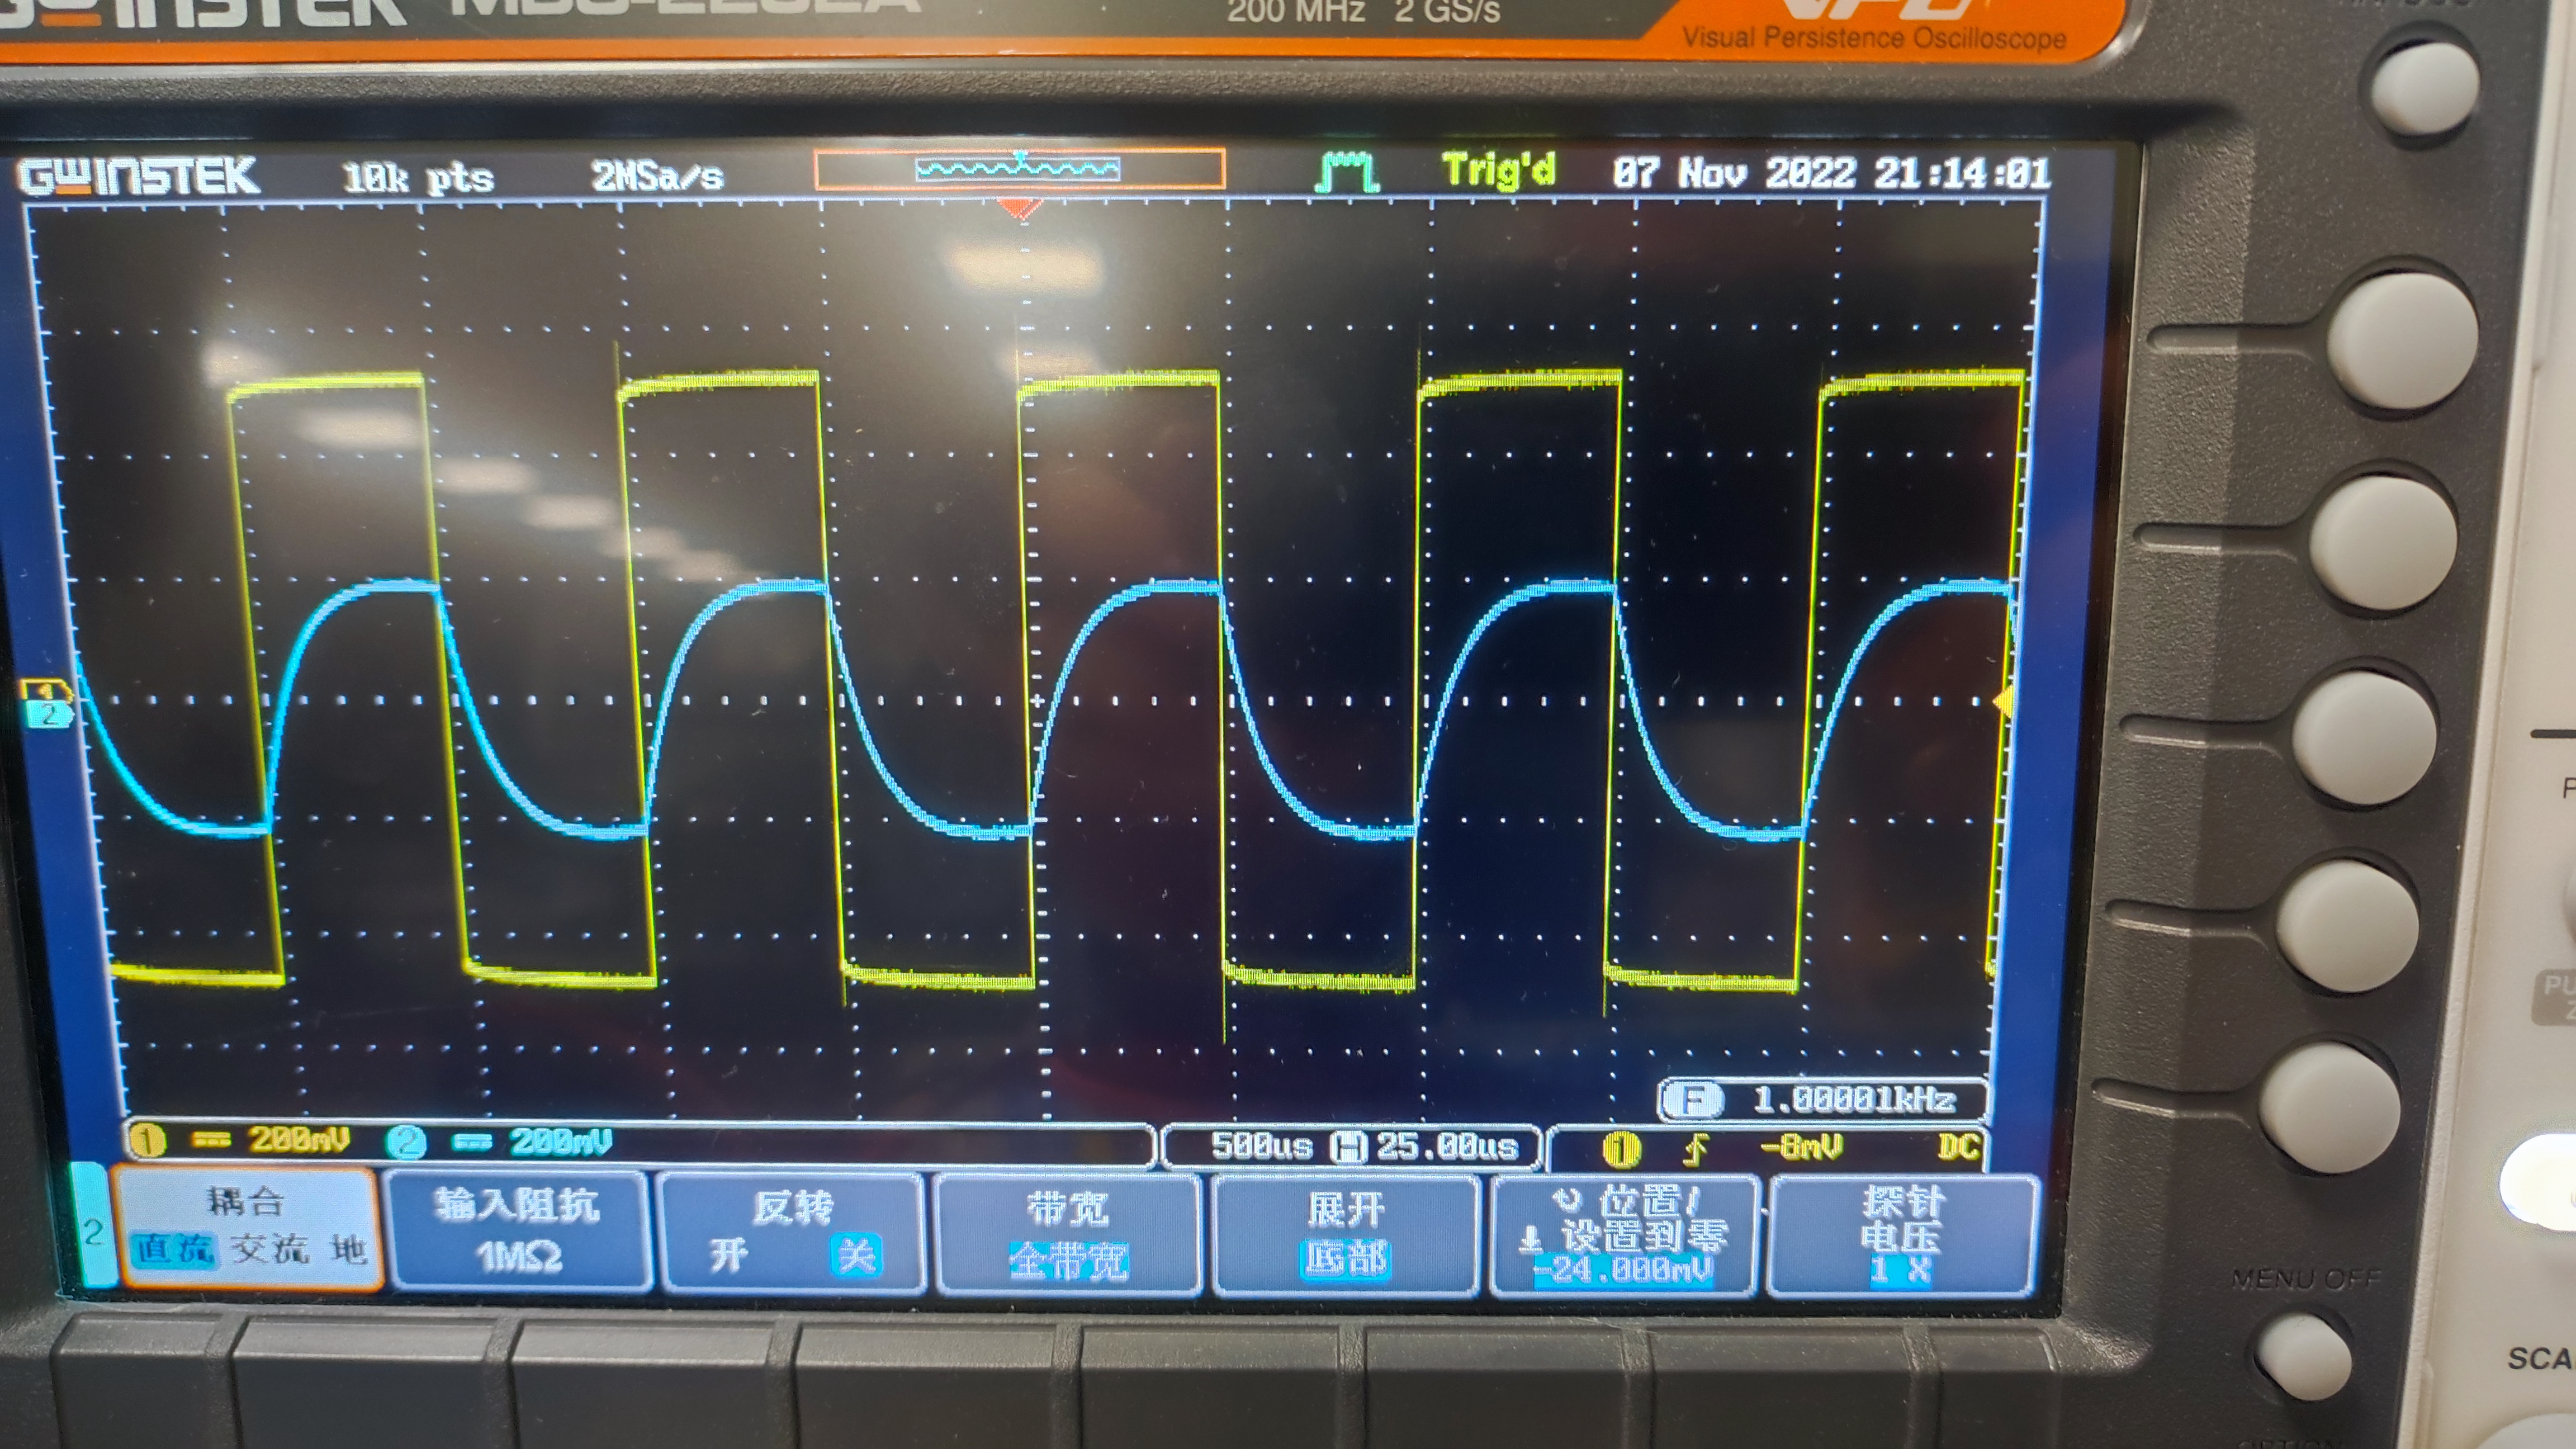
\includegraphics[width=0.9\linewidth]{../图片/滤波器示波器}
			\caption{滤波器示波器图线}
		\end{minipage}		
	\end{figure}
	
	实验时, 使用两个大小为$0.1\mu F$的电容. 为了观察不同大小的电阻对滤波效果的影响, 使用两个滑动变阻器作为电阻. 调节时, 保证两个电阻大小基本相同. 为使$f_0=\frac{1}{2 \pi R C}=$1kHz, 电阻大小理论值为$1591\Omega$. 然而, 由于滑动变阻器大小限制, 当阻值达到最大时, 中心频率仍大于1kHz, 故方波中高频信号基本保留, 部分低频信号被滤除, 仅显示出单边信号滤波效果.
	
	\subsection{文氏震荡电路}
	文氏震荡电路的原理大致为运放的供电电源自激振荡. 其电路图如图所示. 
	
	\begin{figure}[h]
		\centering
		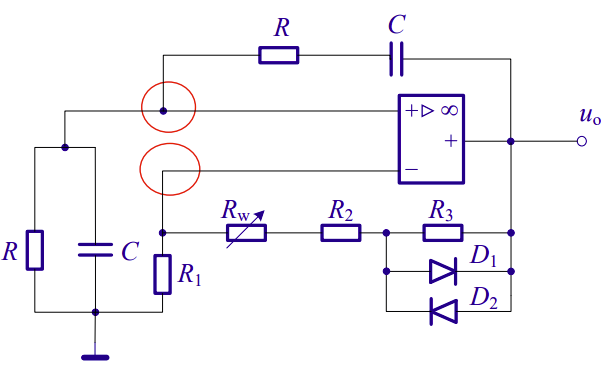
\includegraphics[width=0.3\linewidth]{文氏触发器}
		\caption{文氏触发器}
	\end{figure}

	其中, 两组R, C组成的RC串并网络将输出正反馈至同相输入端, $R_1, R_2$则将输出负反馈至运放的反相输入端, 电路的行为取决于正负反馈较明显的一边. 
	
	通过调节$R_w$可以改变输出波形的幅值大小, 但实际实验时, 由于所需R大小非整数, 实验箱上的两个滑动变阻器都用于调节R的大小, 故实际上未使用改$R_w$. 如不考虑输出波形的频率, 按照原理图接线, 调节$R_w$时, 波形理论上在同一频率上幅值上下变化. 
		
	使用的参数为$R=1k\Omega+$滑动变阻器, $R_1=R_2=R_3=10k\Omega$, $C=0.1\mu F$. 理论上有$f=\frac{1}{2\pi RC}$, 即$R$大约取$1.59k\Omega$. 通过调节滑动变阻器至适当位置使得输出频率恰为1kHz. 示波器波形如图所示. 
	
	\begin{figure}[h]
		\begin{minipage}[t]{0.5\linewidth}
			\centering
			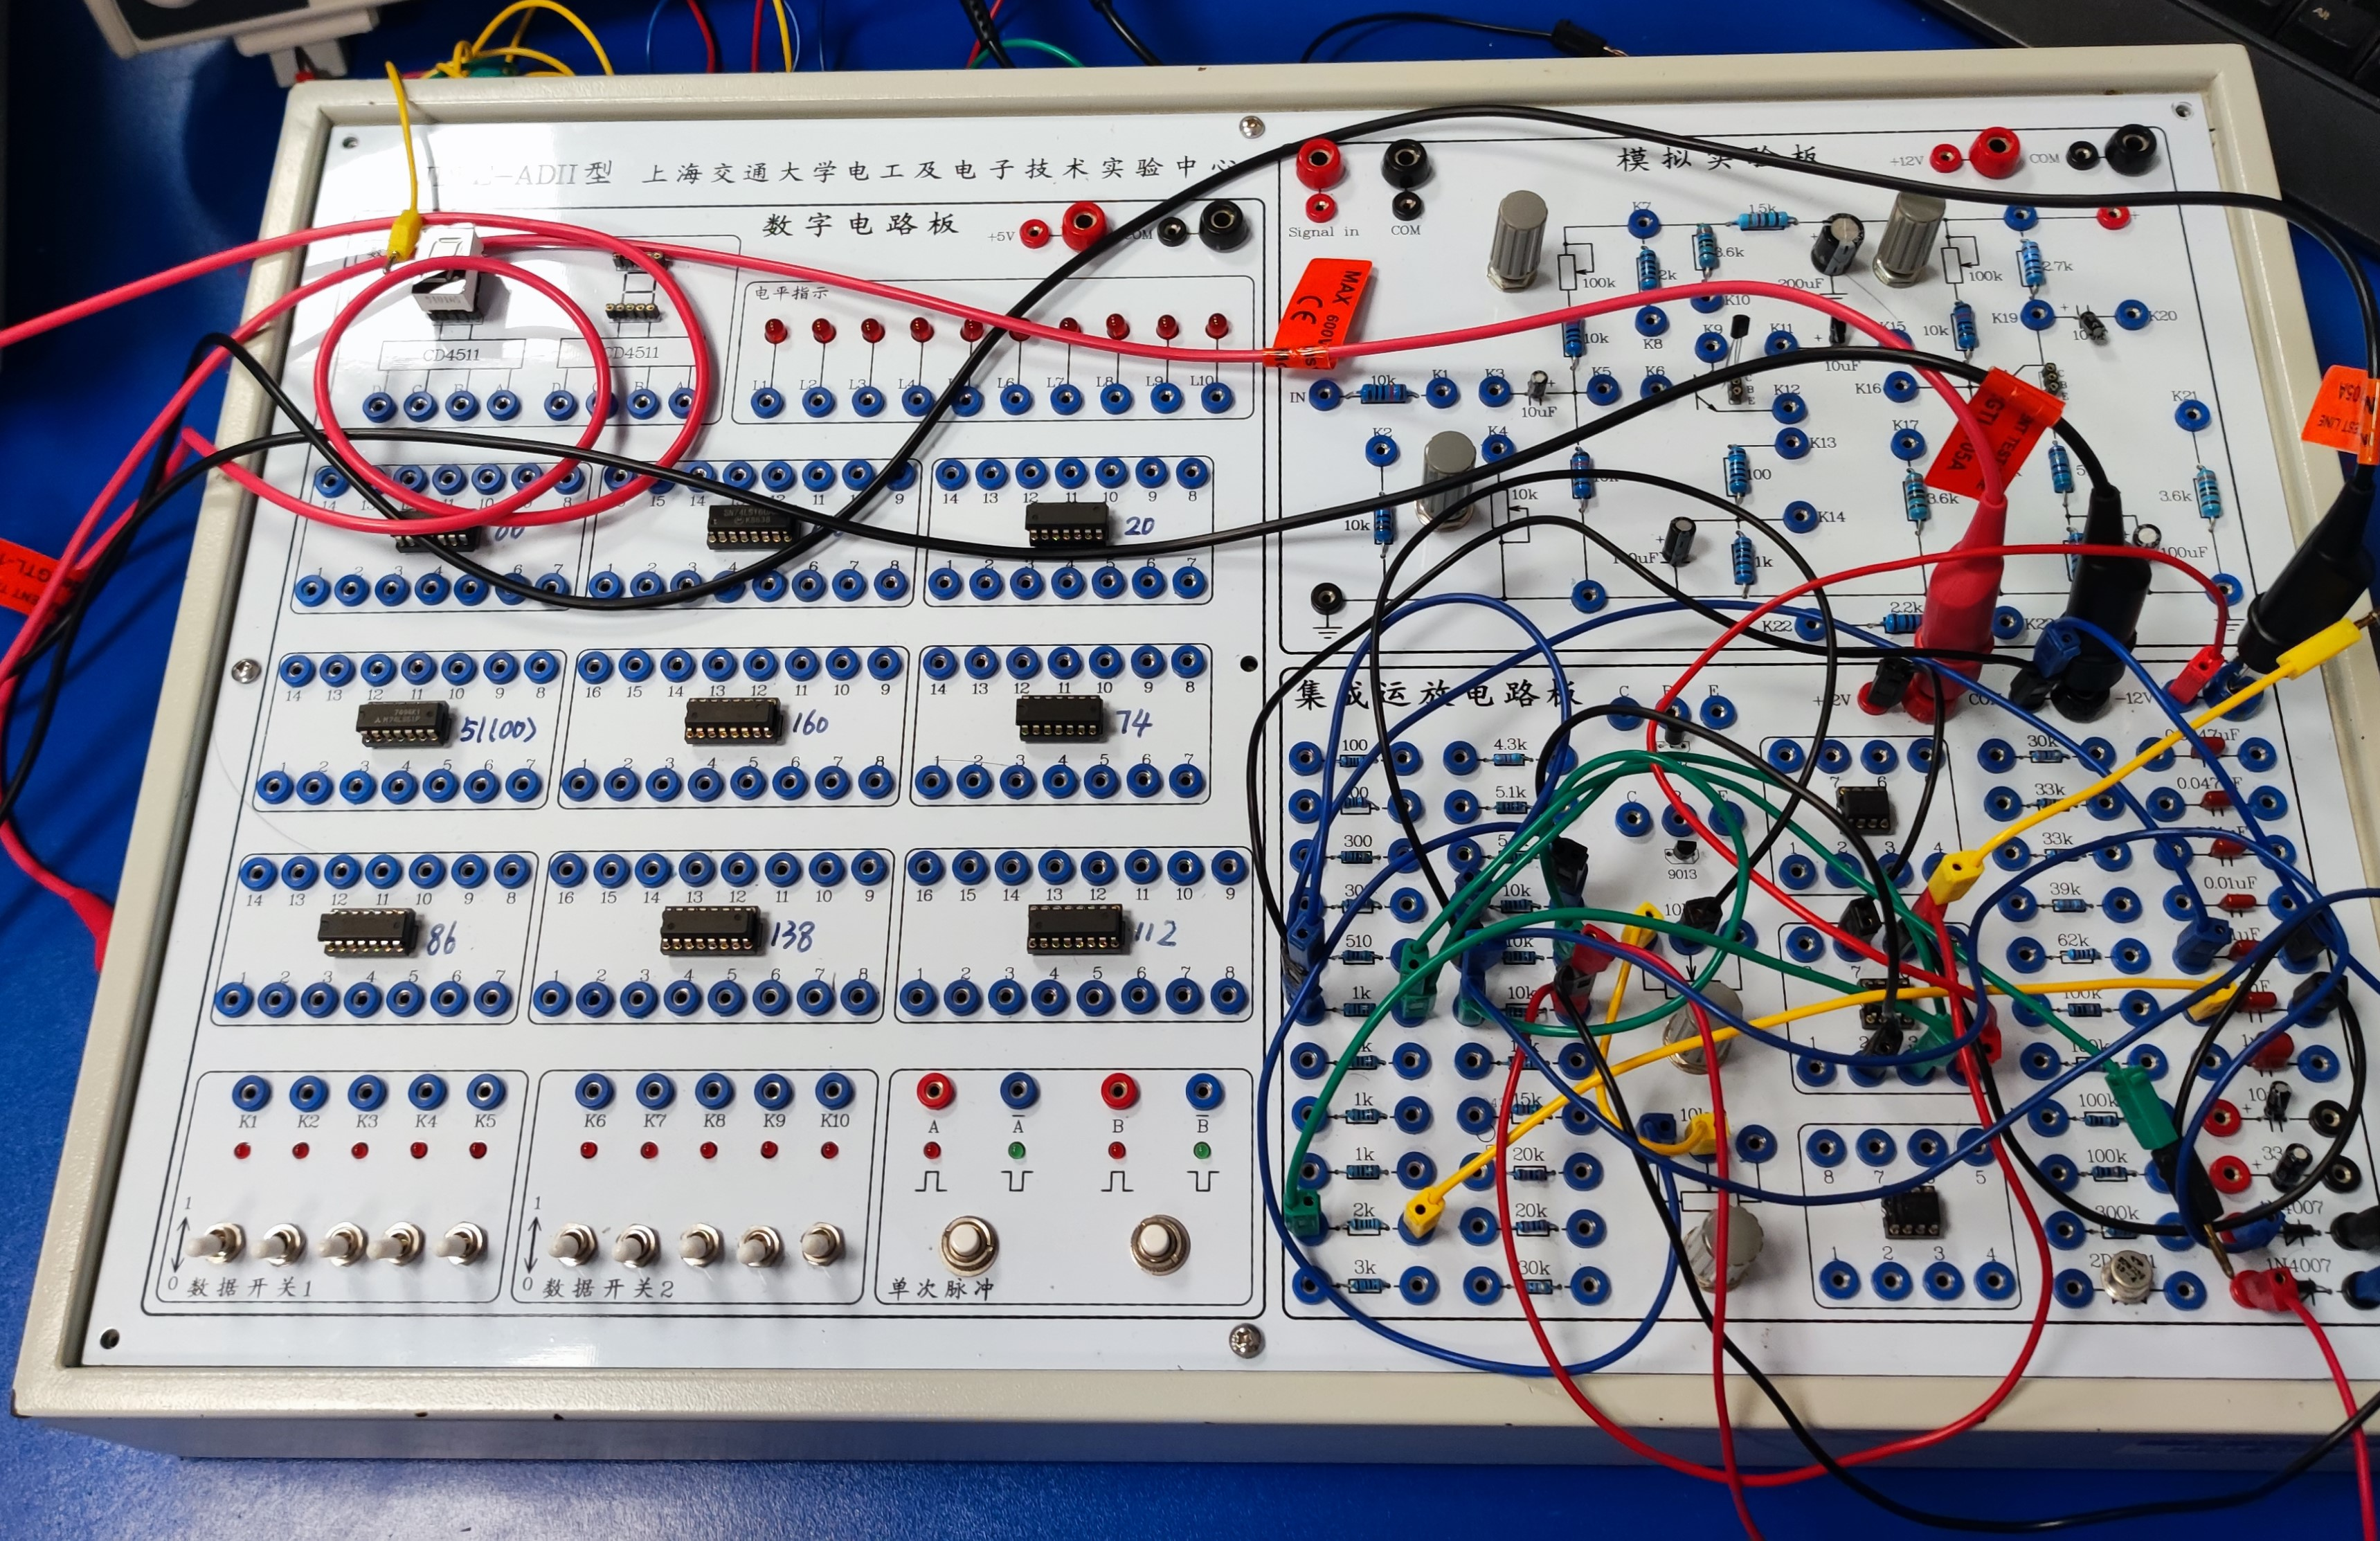
\includegraphics[width=0.9\linewidth]{../图片/文氏发生器连线2}
			\caption{文氏触发器实物图}
		\end{minipage}
		\begin{minipage}[t]{0.5\linewidth}
			\centering
			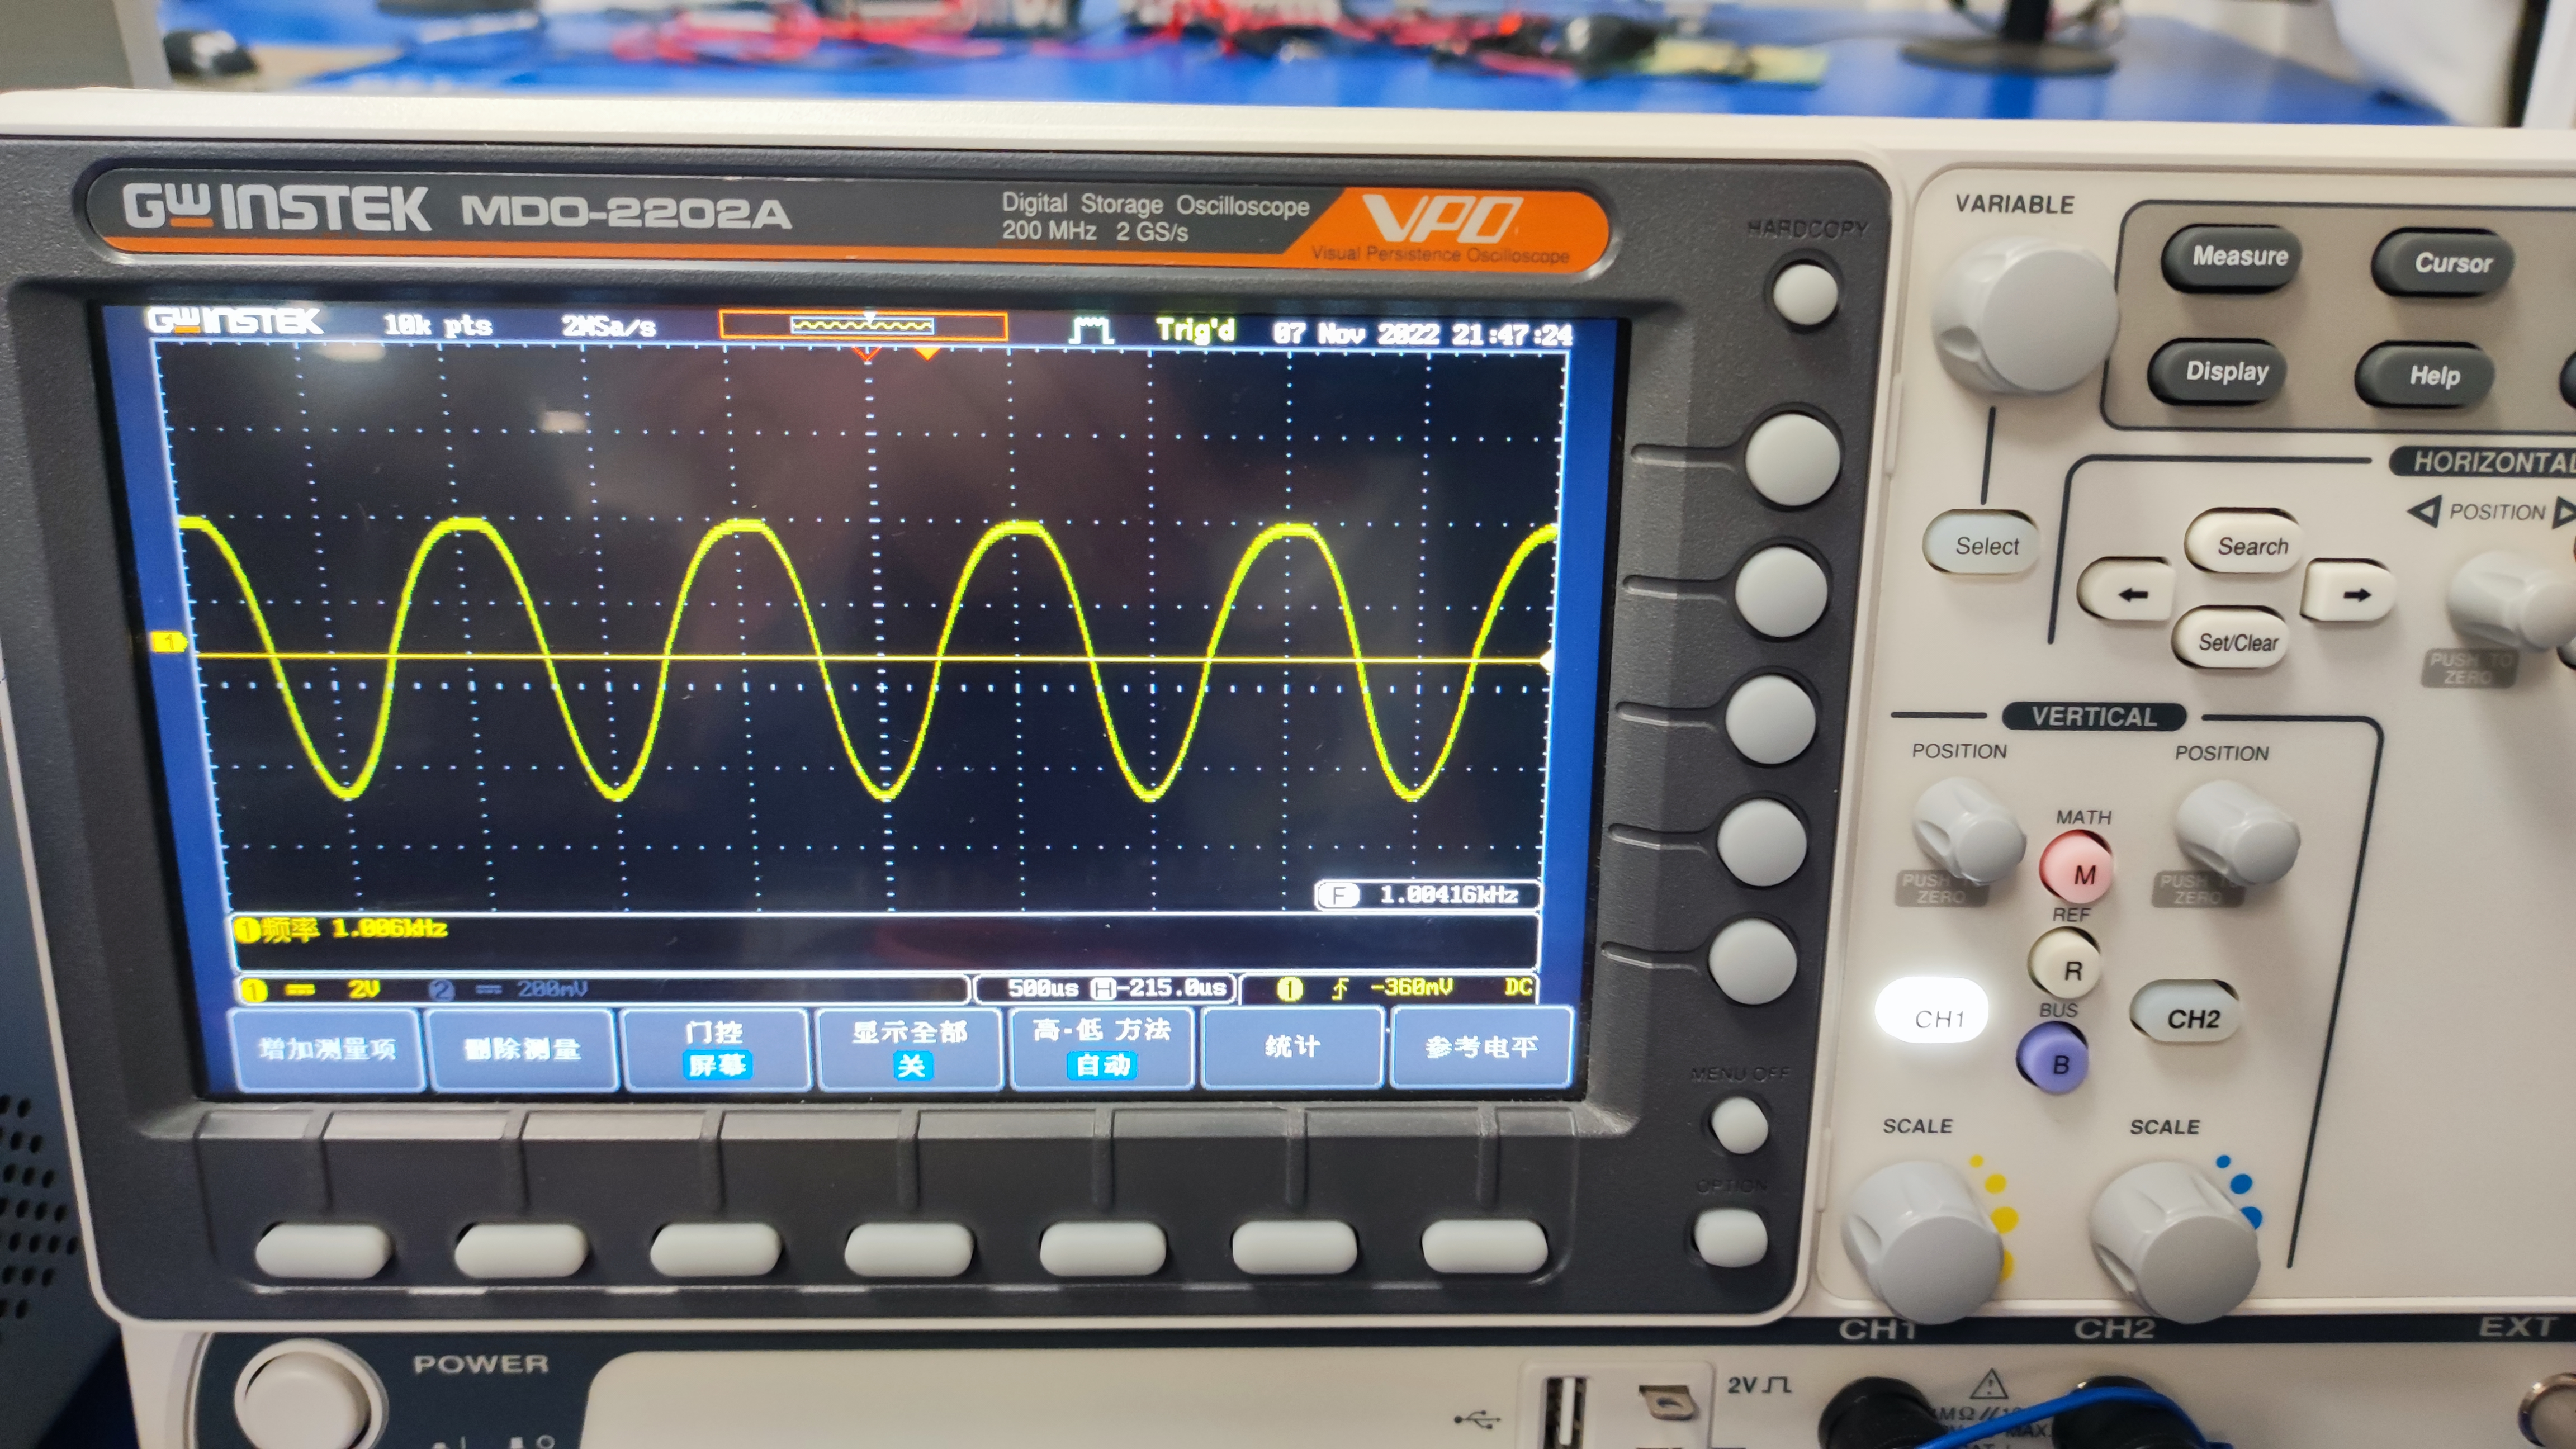
\includegraphics[width=0.9\linewidth]{../图片/文氏触发器示波器}
			\caption{文氏触发器示波器图线}
		\end{minipage}		
	\end{figure}
	
	其中, 两个二极管具有稳压作用, 去除后波形出现更多噪声. 二极管的导通还可使该路上的等效电阻降低, 减小电路波形放大倍数, 避免出现削波失真现象. 去除后$R_2R_3$串联, 放大倍数增加, 可能发生失真. 
	
	\subsection{方波、三角波发生电路}
	方波三角波发生器电路如图所示. 实际上只需实现三角波, 加上积分器后就能产生方波. 因此该实验需要两块UA741芯片. 
	
	\begin{figure}[h]
		\centering
		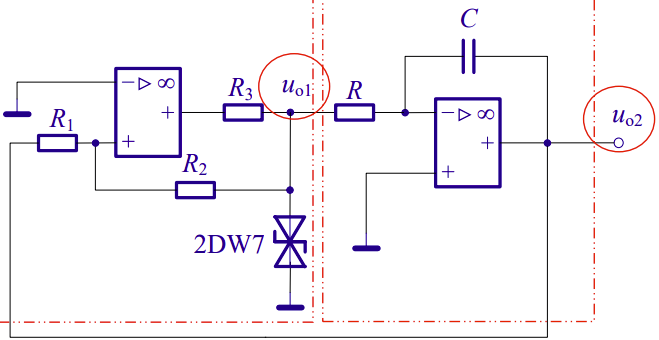
\includegraphics[width=0.3\linewidth]{方波三角波发生器}
		\caption{方波三角波发生器}
	\end{figure}

	分析该电路, 该电路关系复杂, 难以直接列写方程. 故实验时使用不同阻值的电阻进行了测试. 测试结果是在$R_1=1k\Omega,~R_2=20k\Omega,~R_3=R=10k\Omega$, 输出了约为400Hz的波形. 输出波形如图所示. 连接滑动变阻器, 理论上可以使得频率取得更接近500Hz的结果. 
	
	\begin{figure}[h]
		\begin{minipage}[t]{0.5\linewidth}
			\centering
			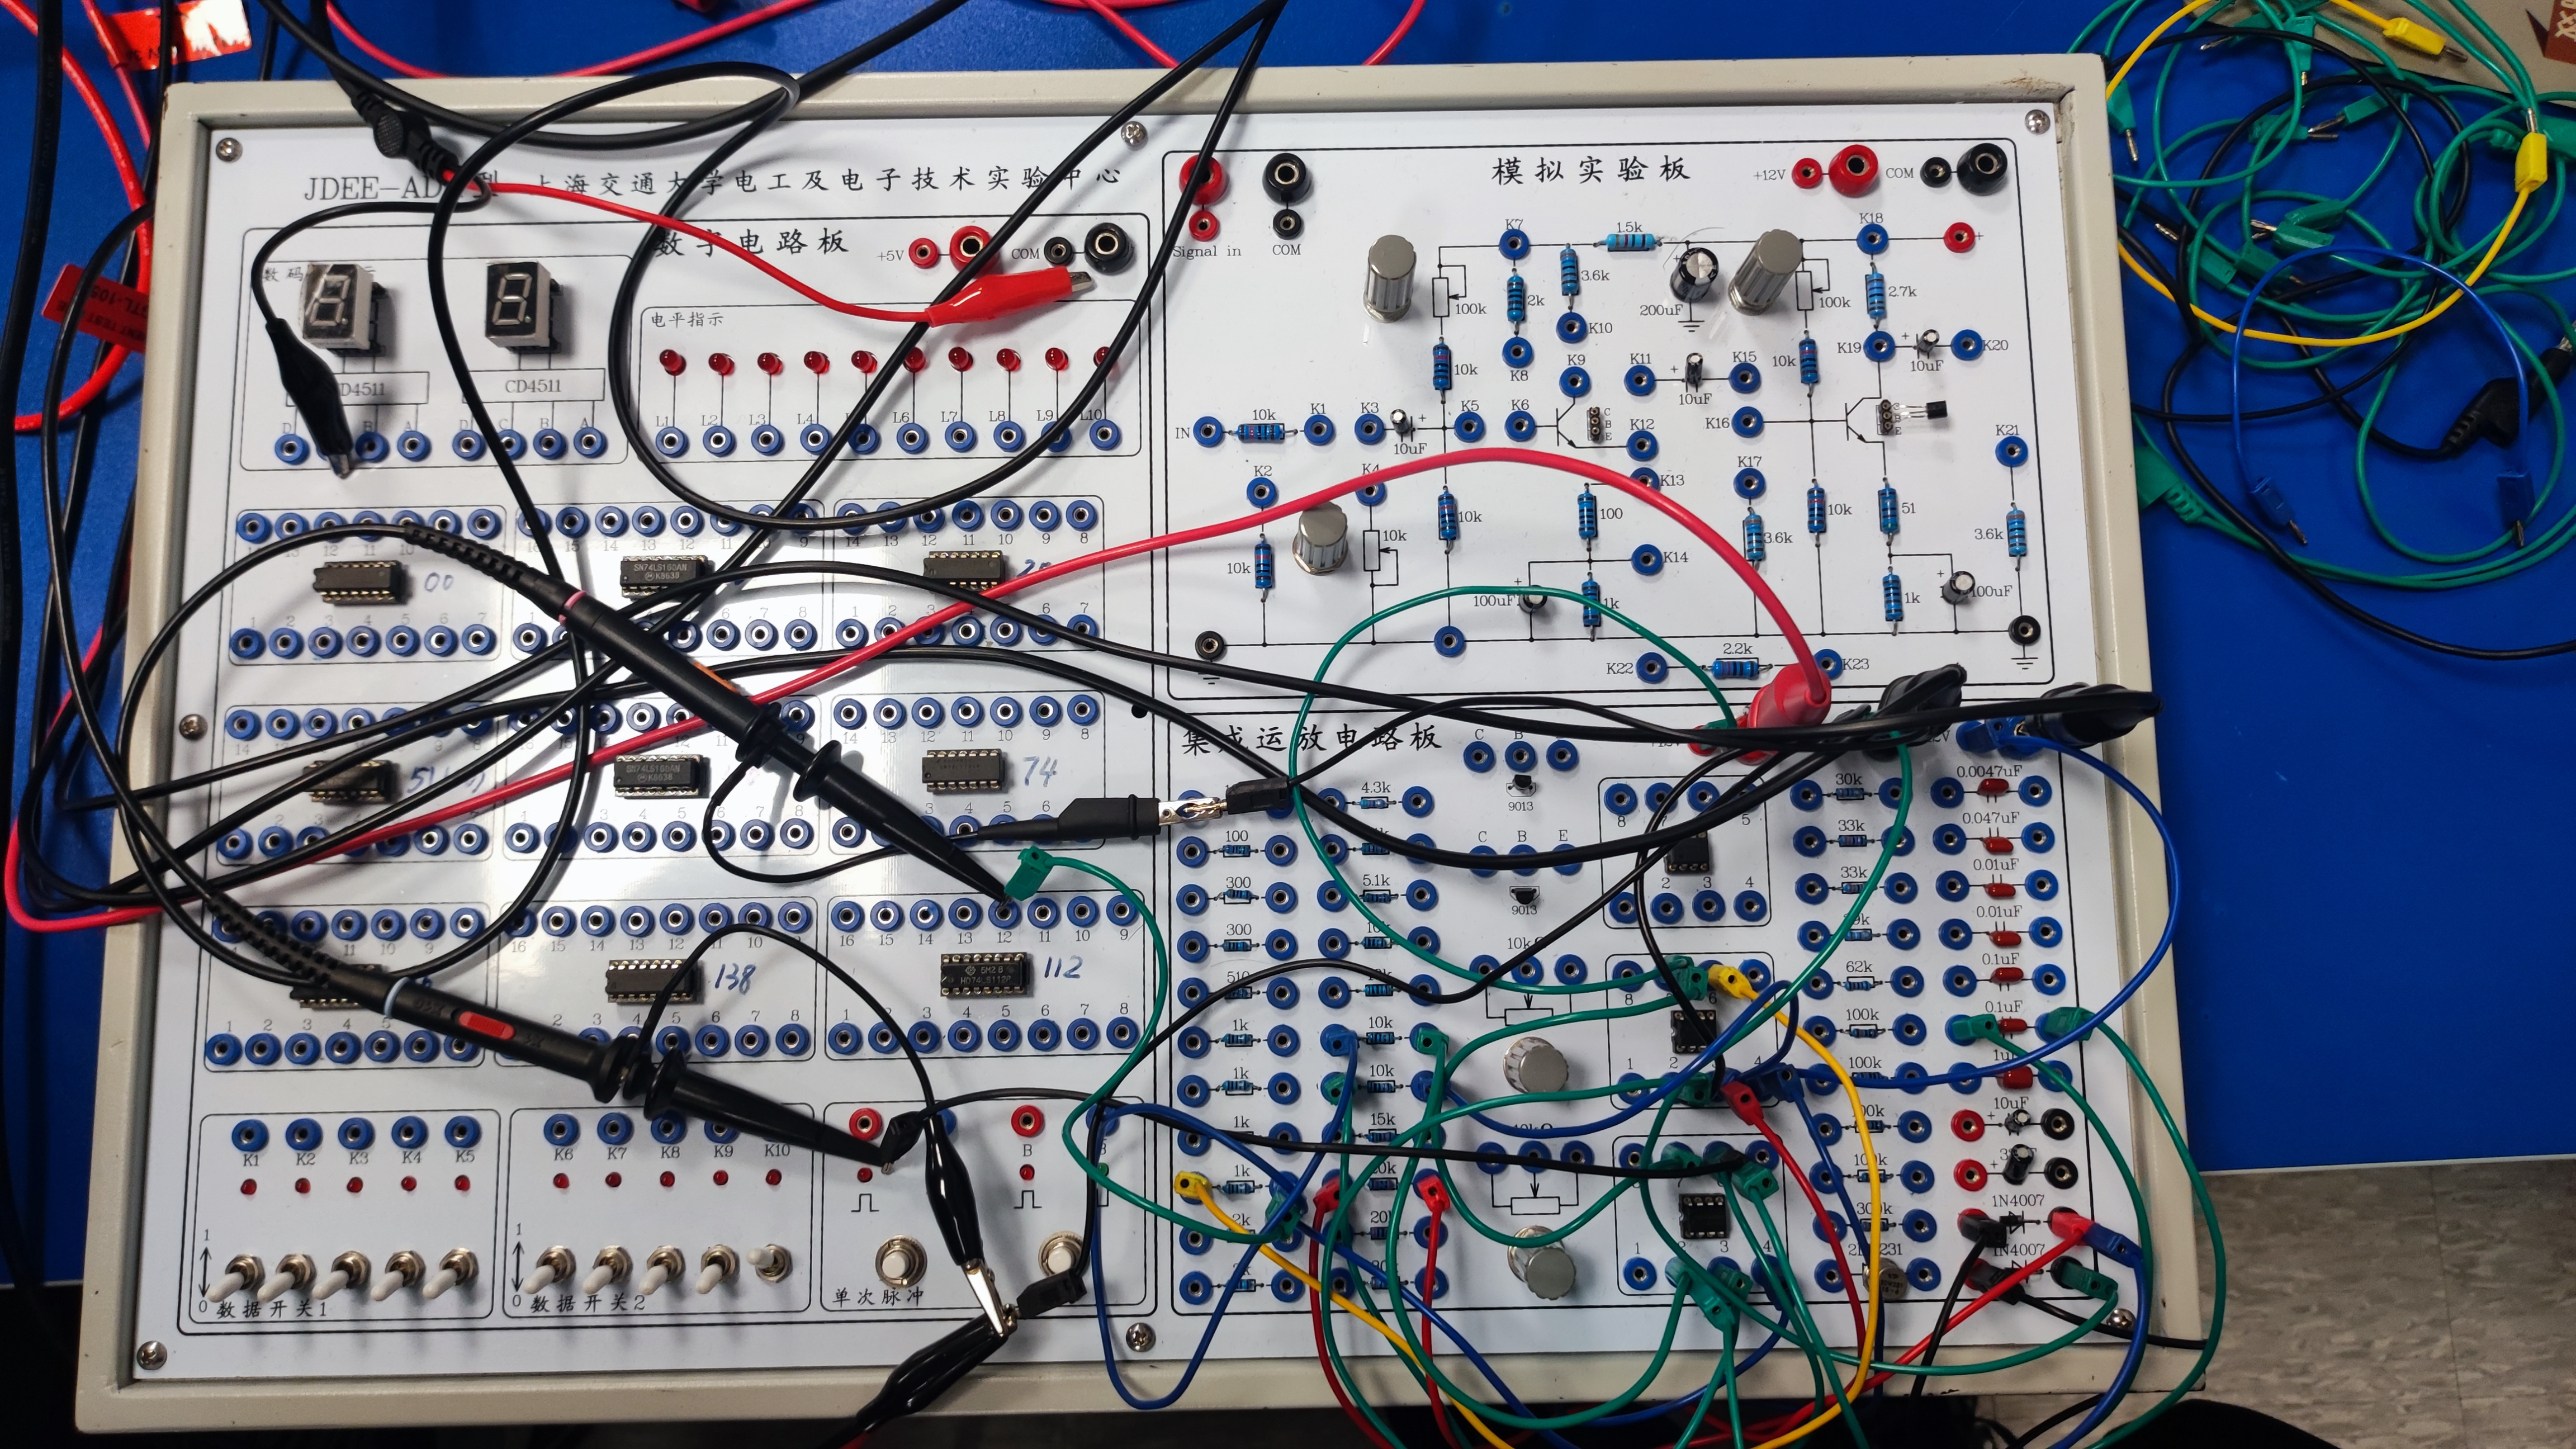
\includegraphics[width=0.9\linewidth]{../图片/波形发生器连线}
			\caption{波形发生器实物图}
		\end{minipage}
		\begin{minipage}[t]{0.5\linewidth}
			\centering
			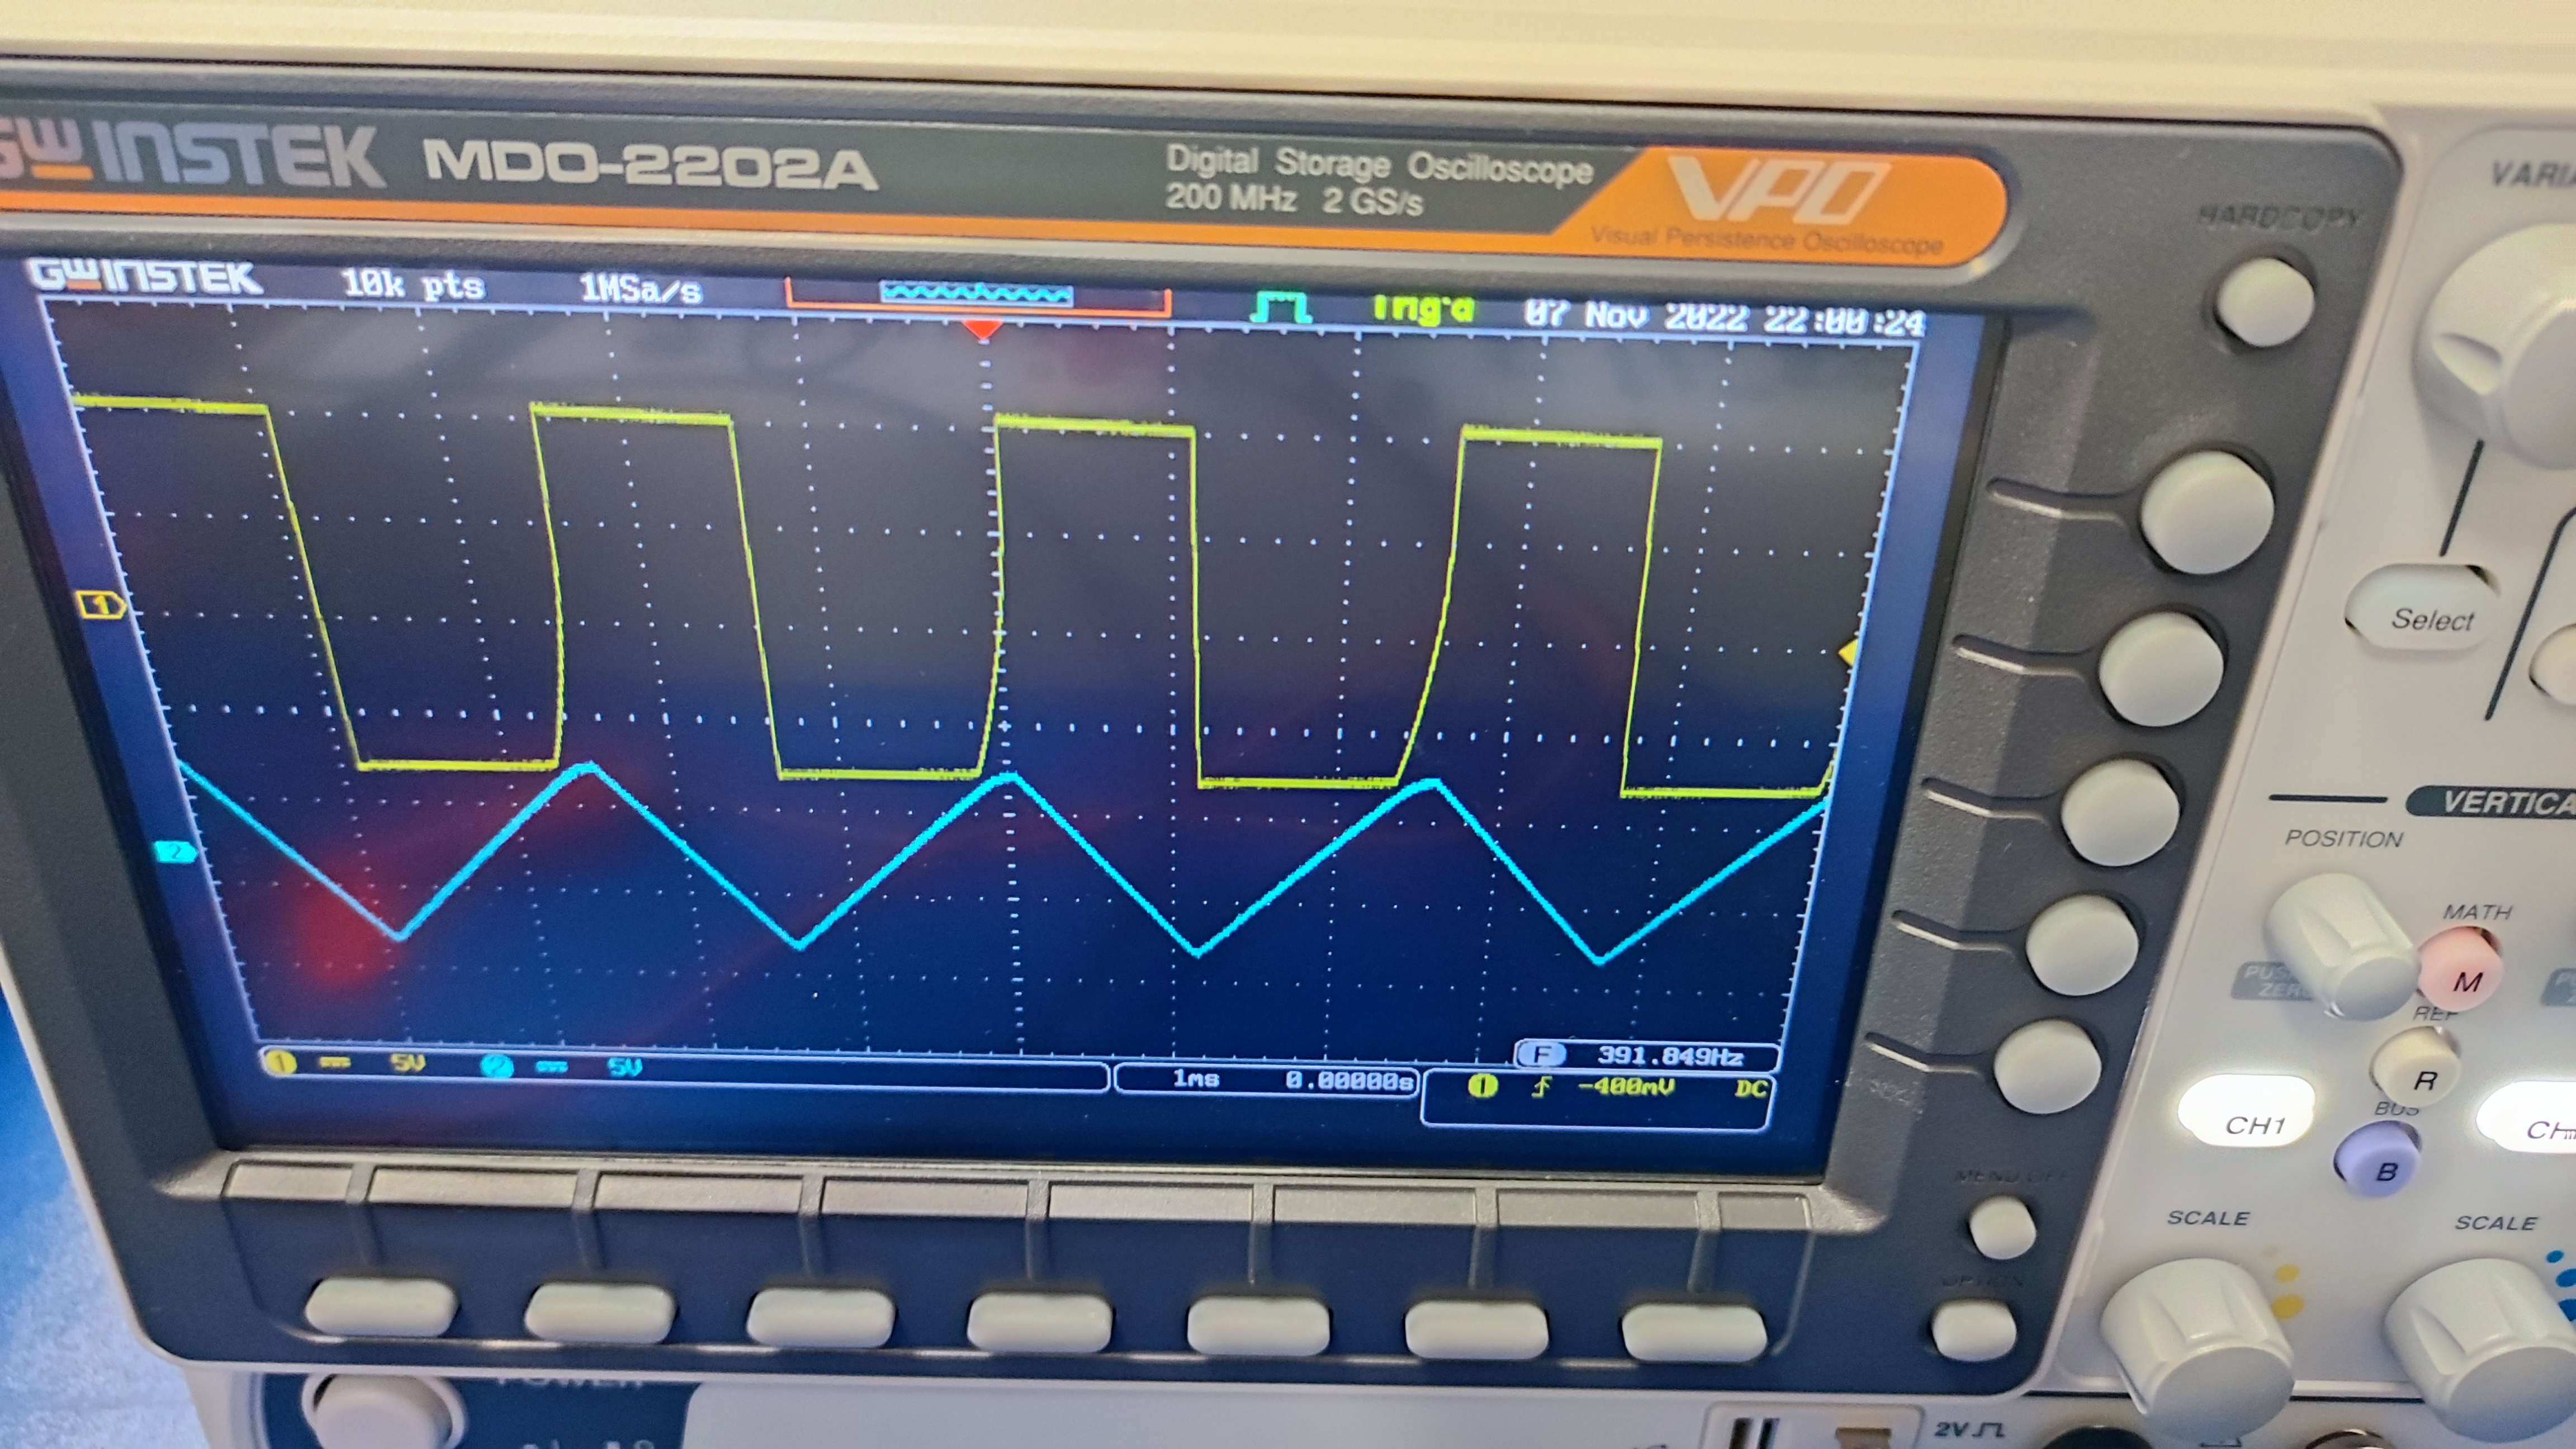
\includegraphics[width=0.9\linewidth]{../图片/波形发生器示波器}
			\caption{波形发生器示波器图线}
		\end{minipage}		
	\end{figure}

	\subsection{555定时器构成施密特触发器}
	施密特触发器有回差电压特性, 能将边沿变化缓慢的电压波形整形为边沿陡峭的矩形脉冲. 555定时器构成的施密特触发器是一种具有两个稳态的电路. 当输入电压大于电路导通电压时, 输出维持于一个恒定的电压值, 当输入电压低于电路截止电压时, 输出维持于另一个恒定的电压值. 它是一种脉冲整形电, 用于脉冲波形的变换和整形, 是一种双稳电路. 使用555触发器设计施密特触发器, 电路如图所示. 555触发器使用5V供电. 
	
	\begin{figure}[h]
		\centering
		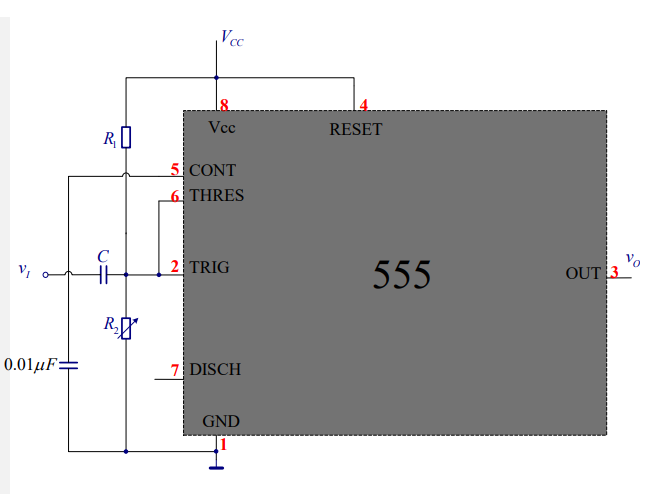
\includegraphics[width=0.6\linewidth]{555触发器}
		\caption{555触发器}
	\end{figure}


	
	如图所示, 电容大小为$0.01\mu F$, R1大小为$50\Omega$. R2使用滑动变阻器. 输入信号为500Hz, 3Vpp的正弦交流信号. 输出信号频率也为500Hz, 是方波信号. 调节滑动变阻器大小可以使占空比发生变化. 
	
	555触发器实物图如图所示. 图片还显示了不同电阻下占空比的变化.
	
	\begin{figure}[h]
		\begin{minipage}[t]{0.5\linewidth}
			\centering
			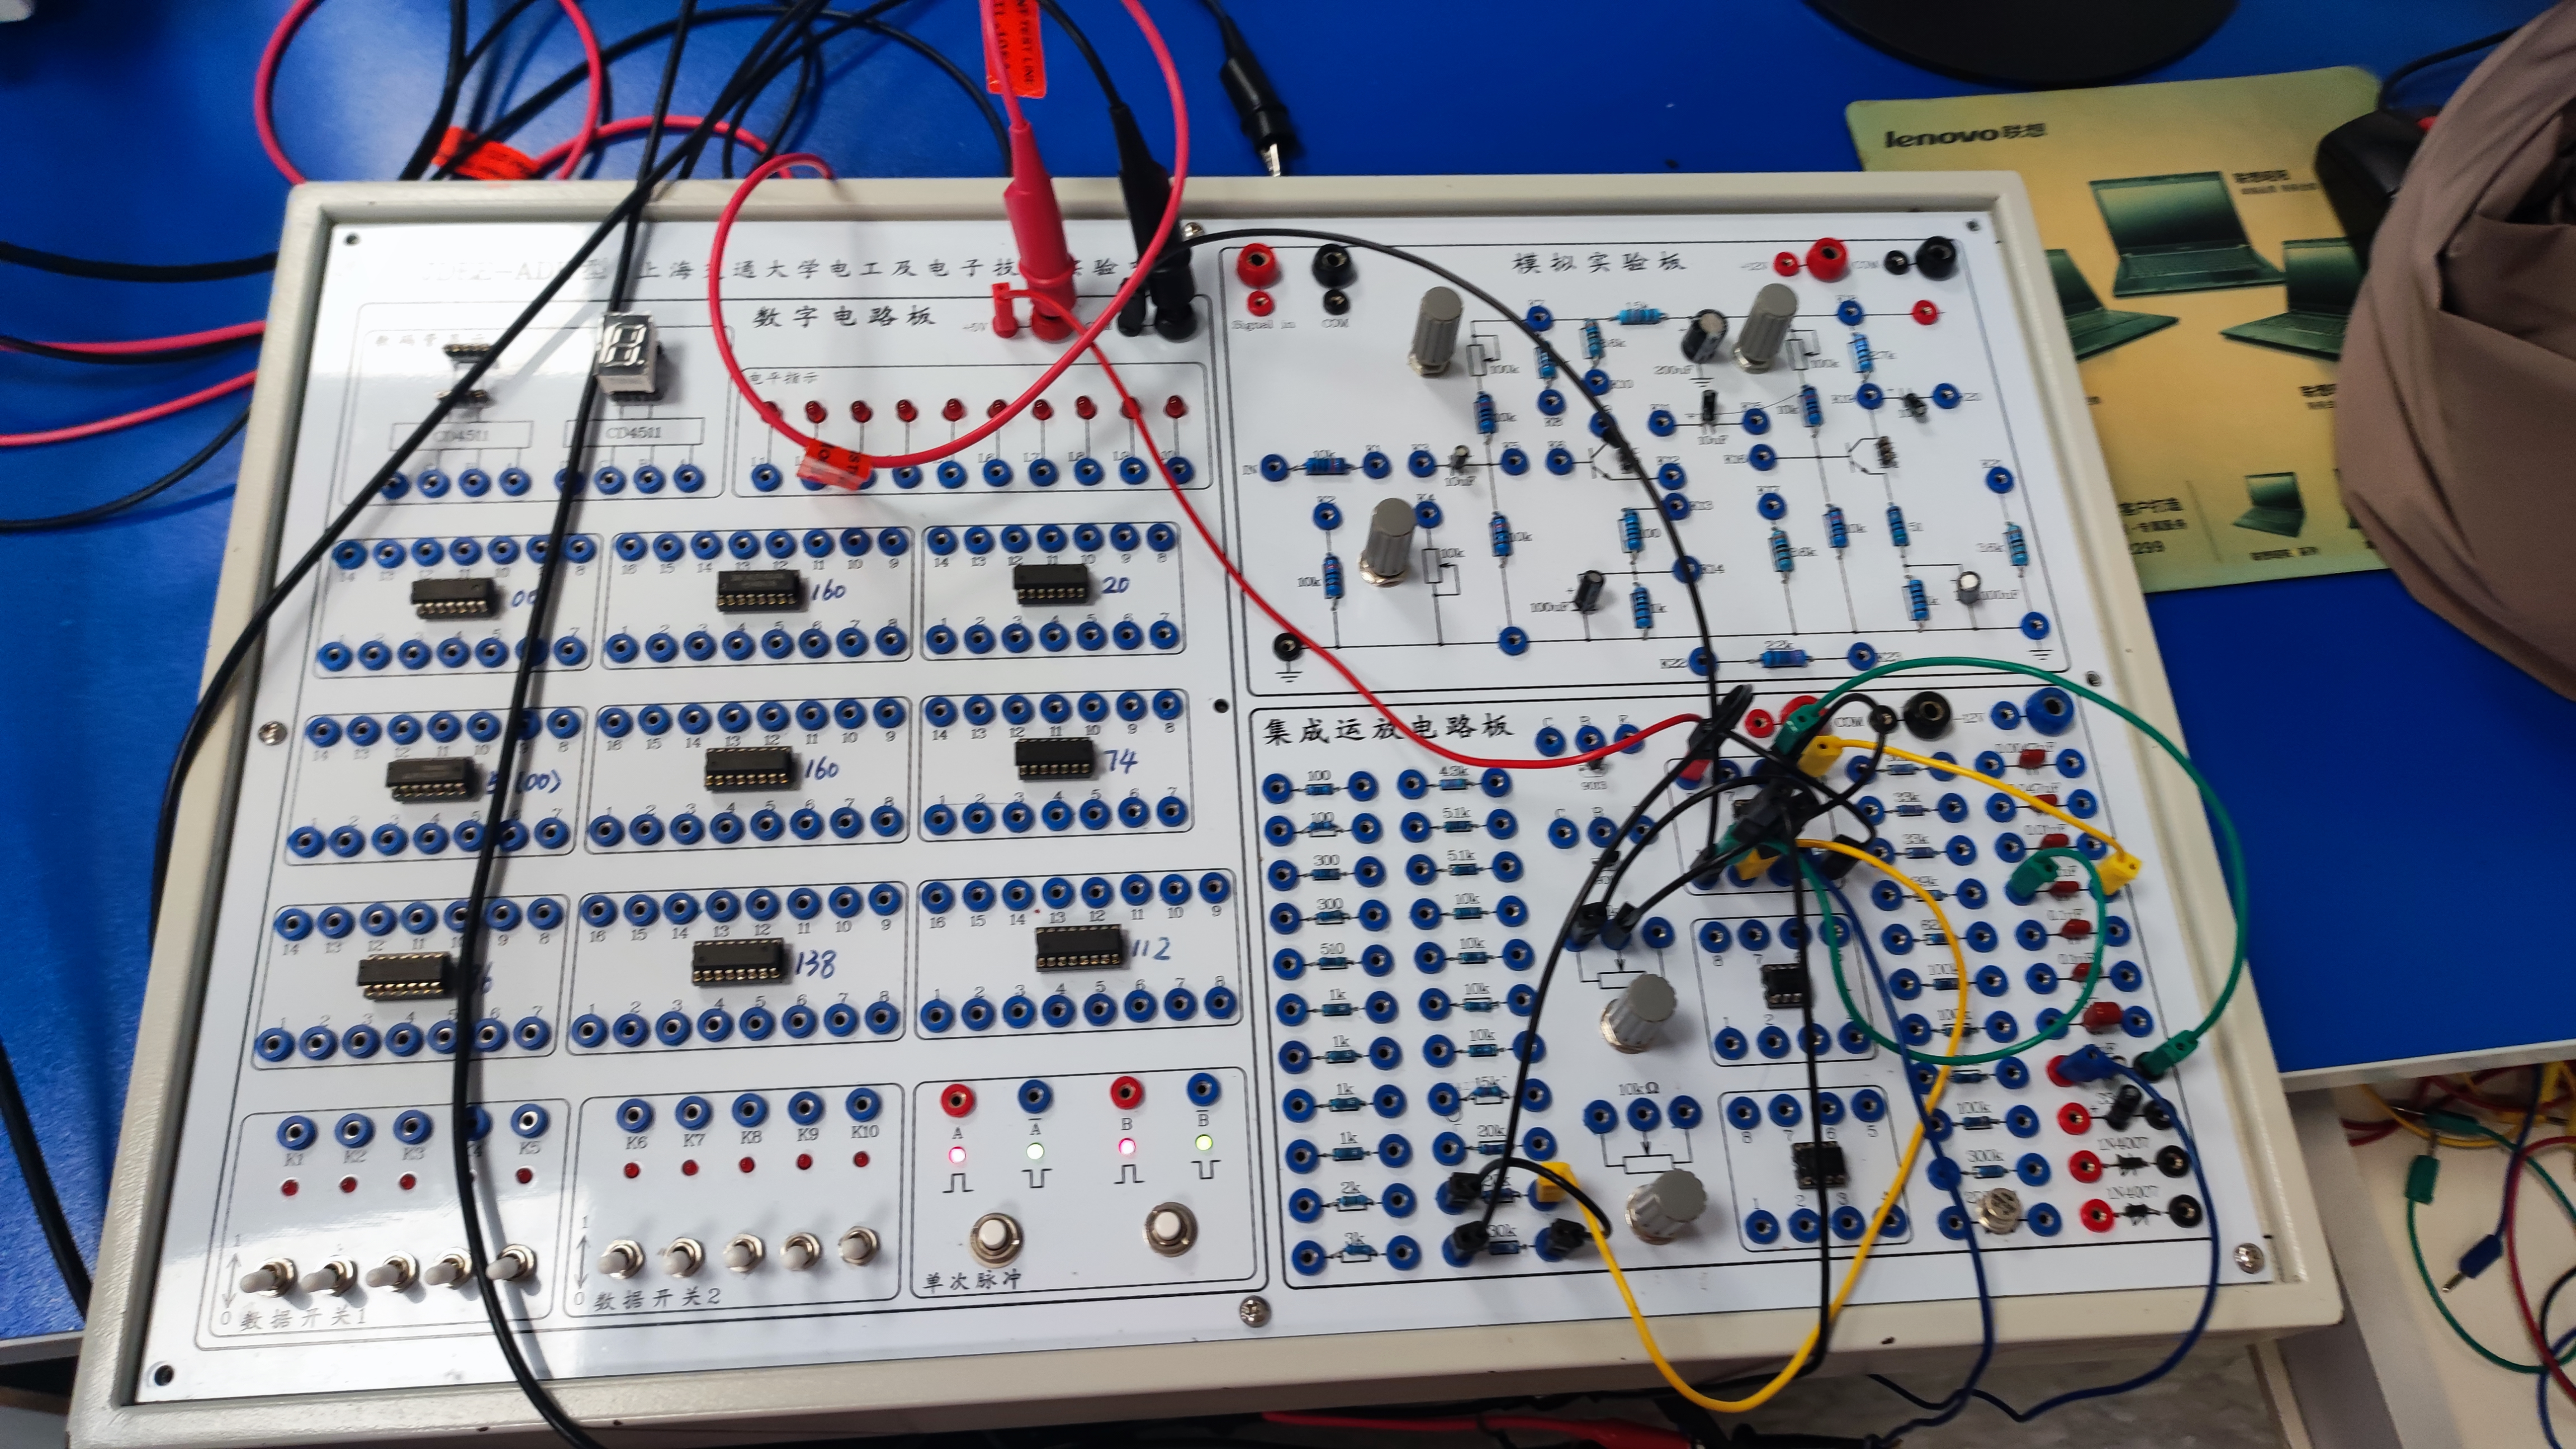
\includegraphics[width=0.9\linewidth]{../图片/555触发器连线}
			\caption{555触发器连线}
		\end{minipage}
		\begin{minipage}[t]{0.5\linewidth}
			\centering
			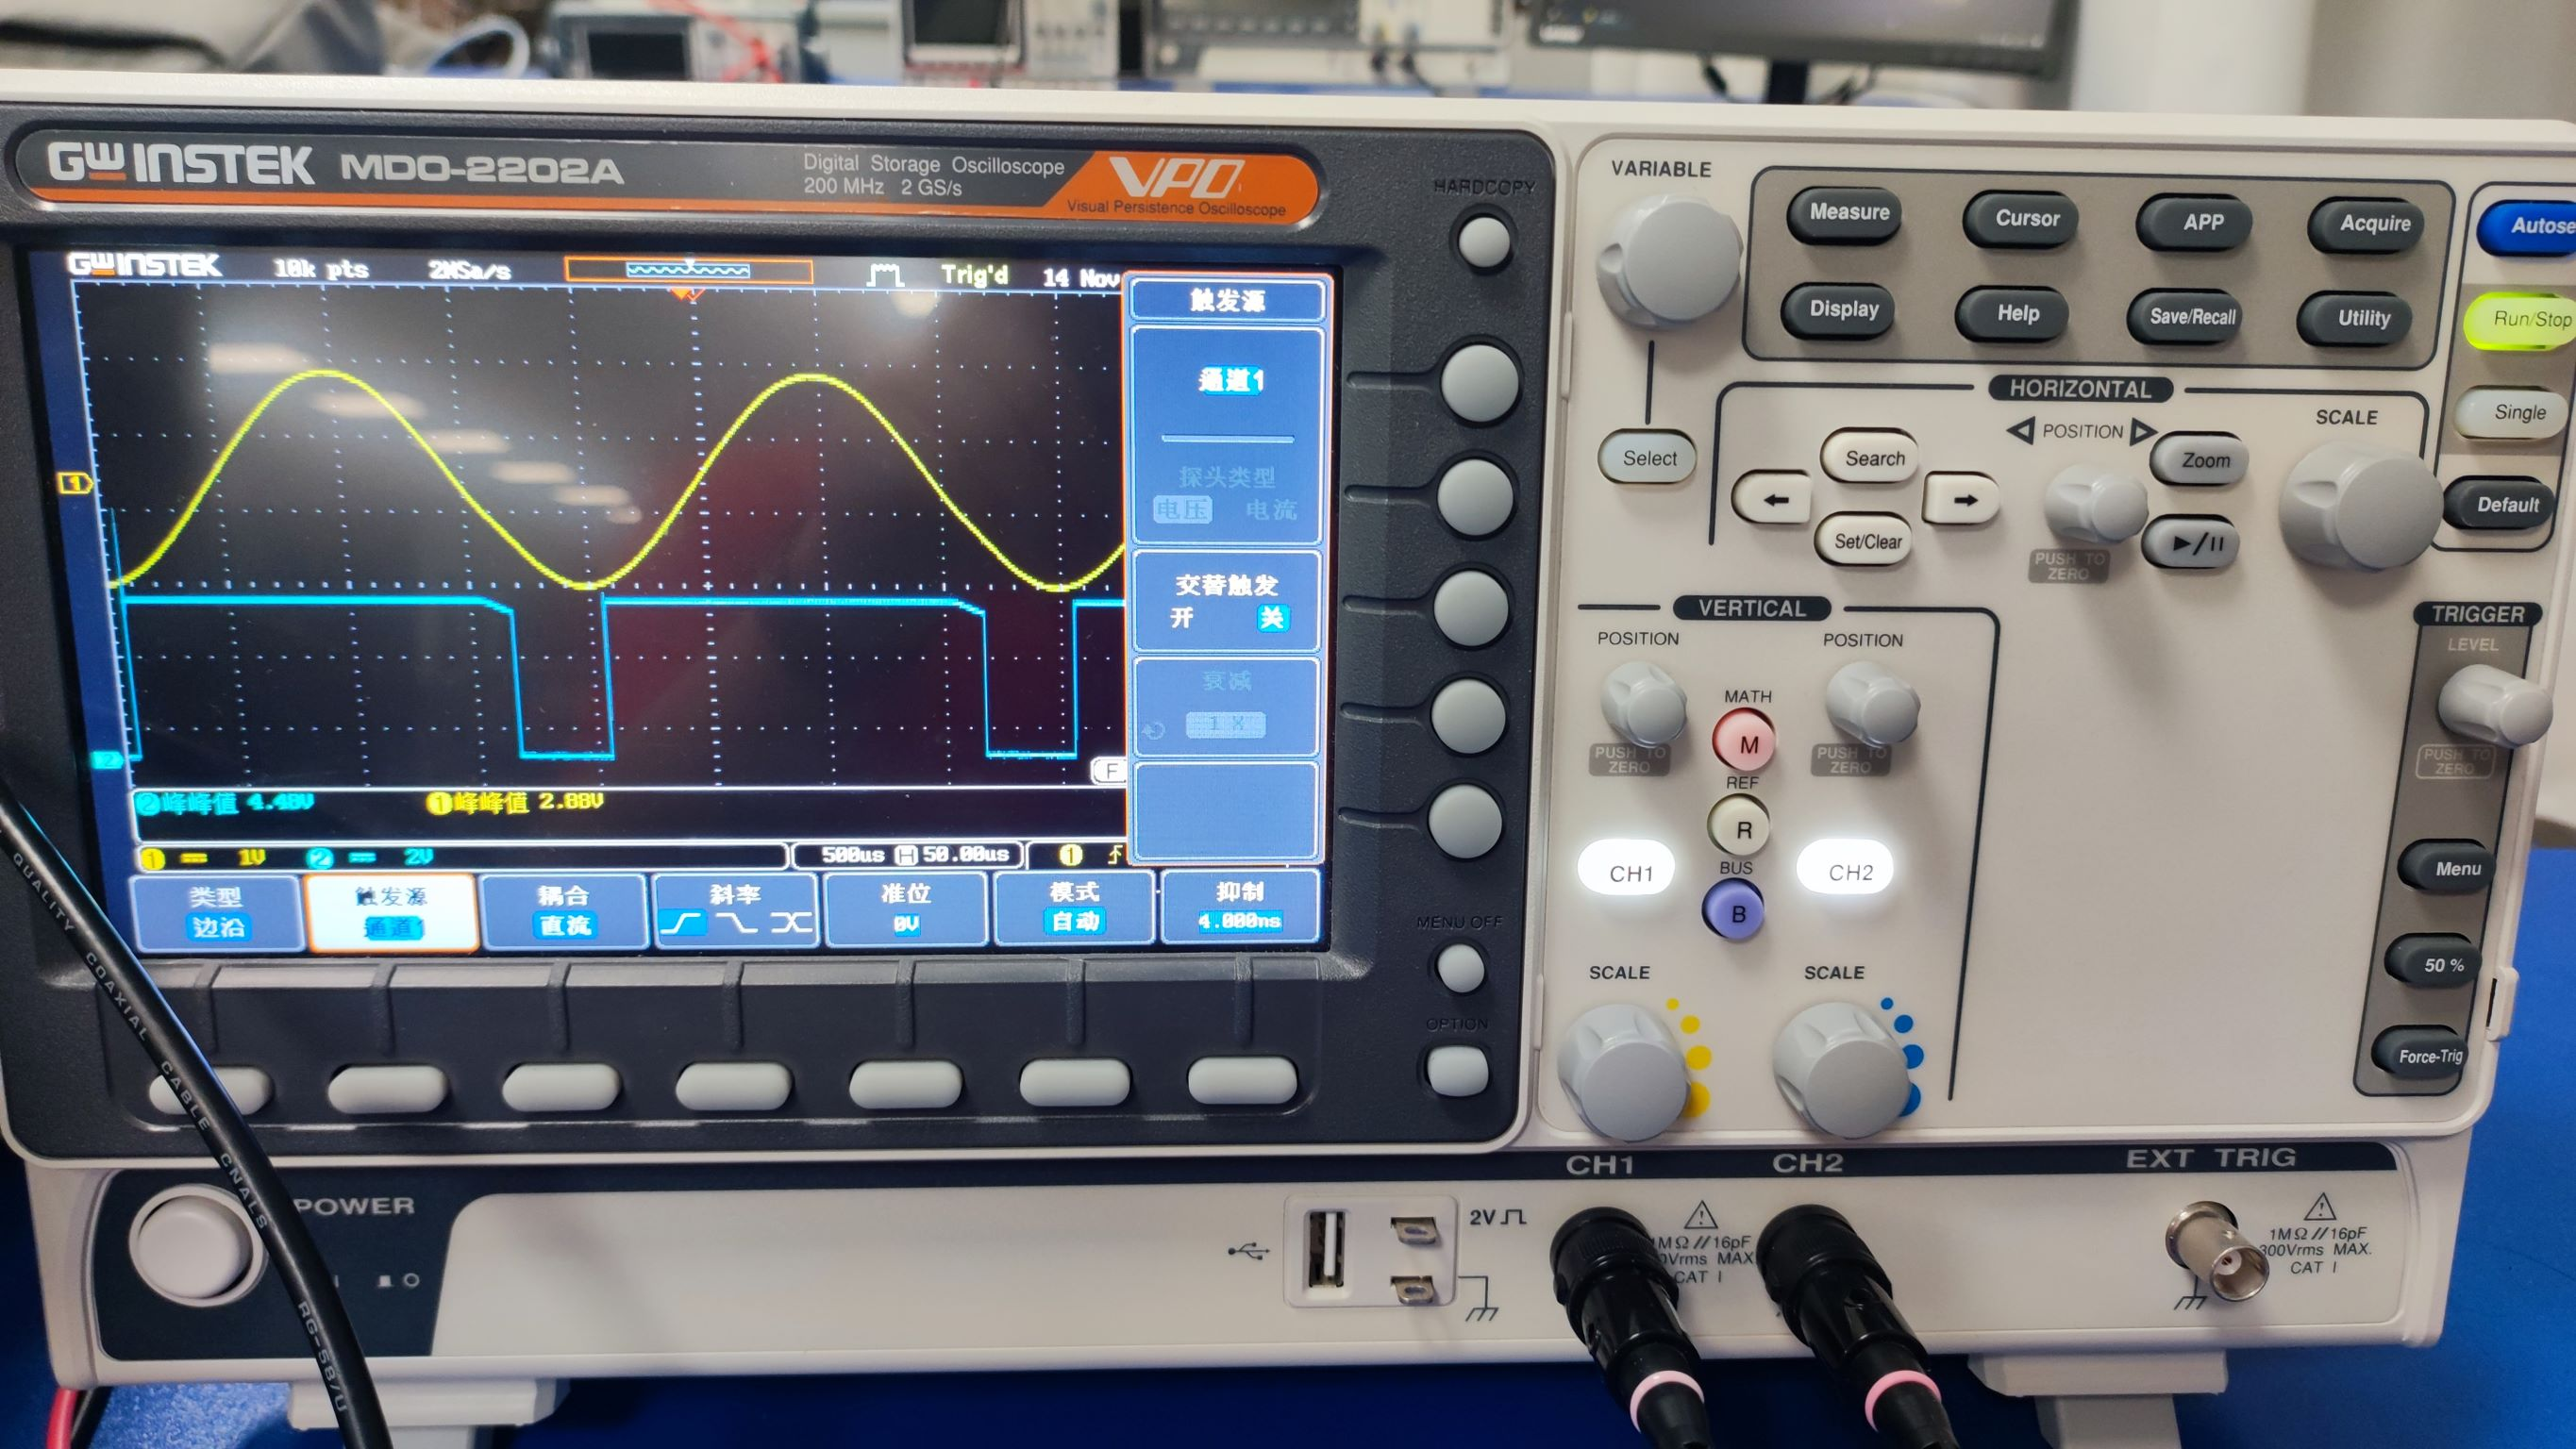
\includegraphics[width=0.9\linewidth]{../图片/555示波器1}
			\caption{555示波器1}
		\end{minipage}		
		\begin{minipage}[t]{0.5\linewidth}
			\centering
			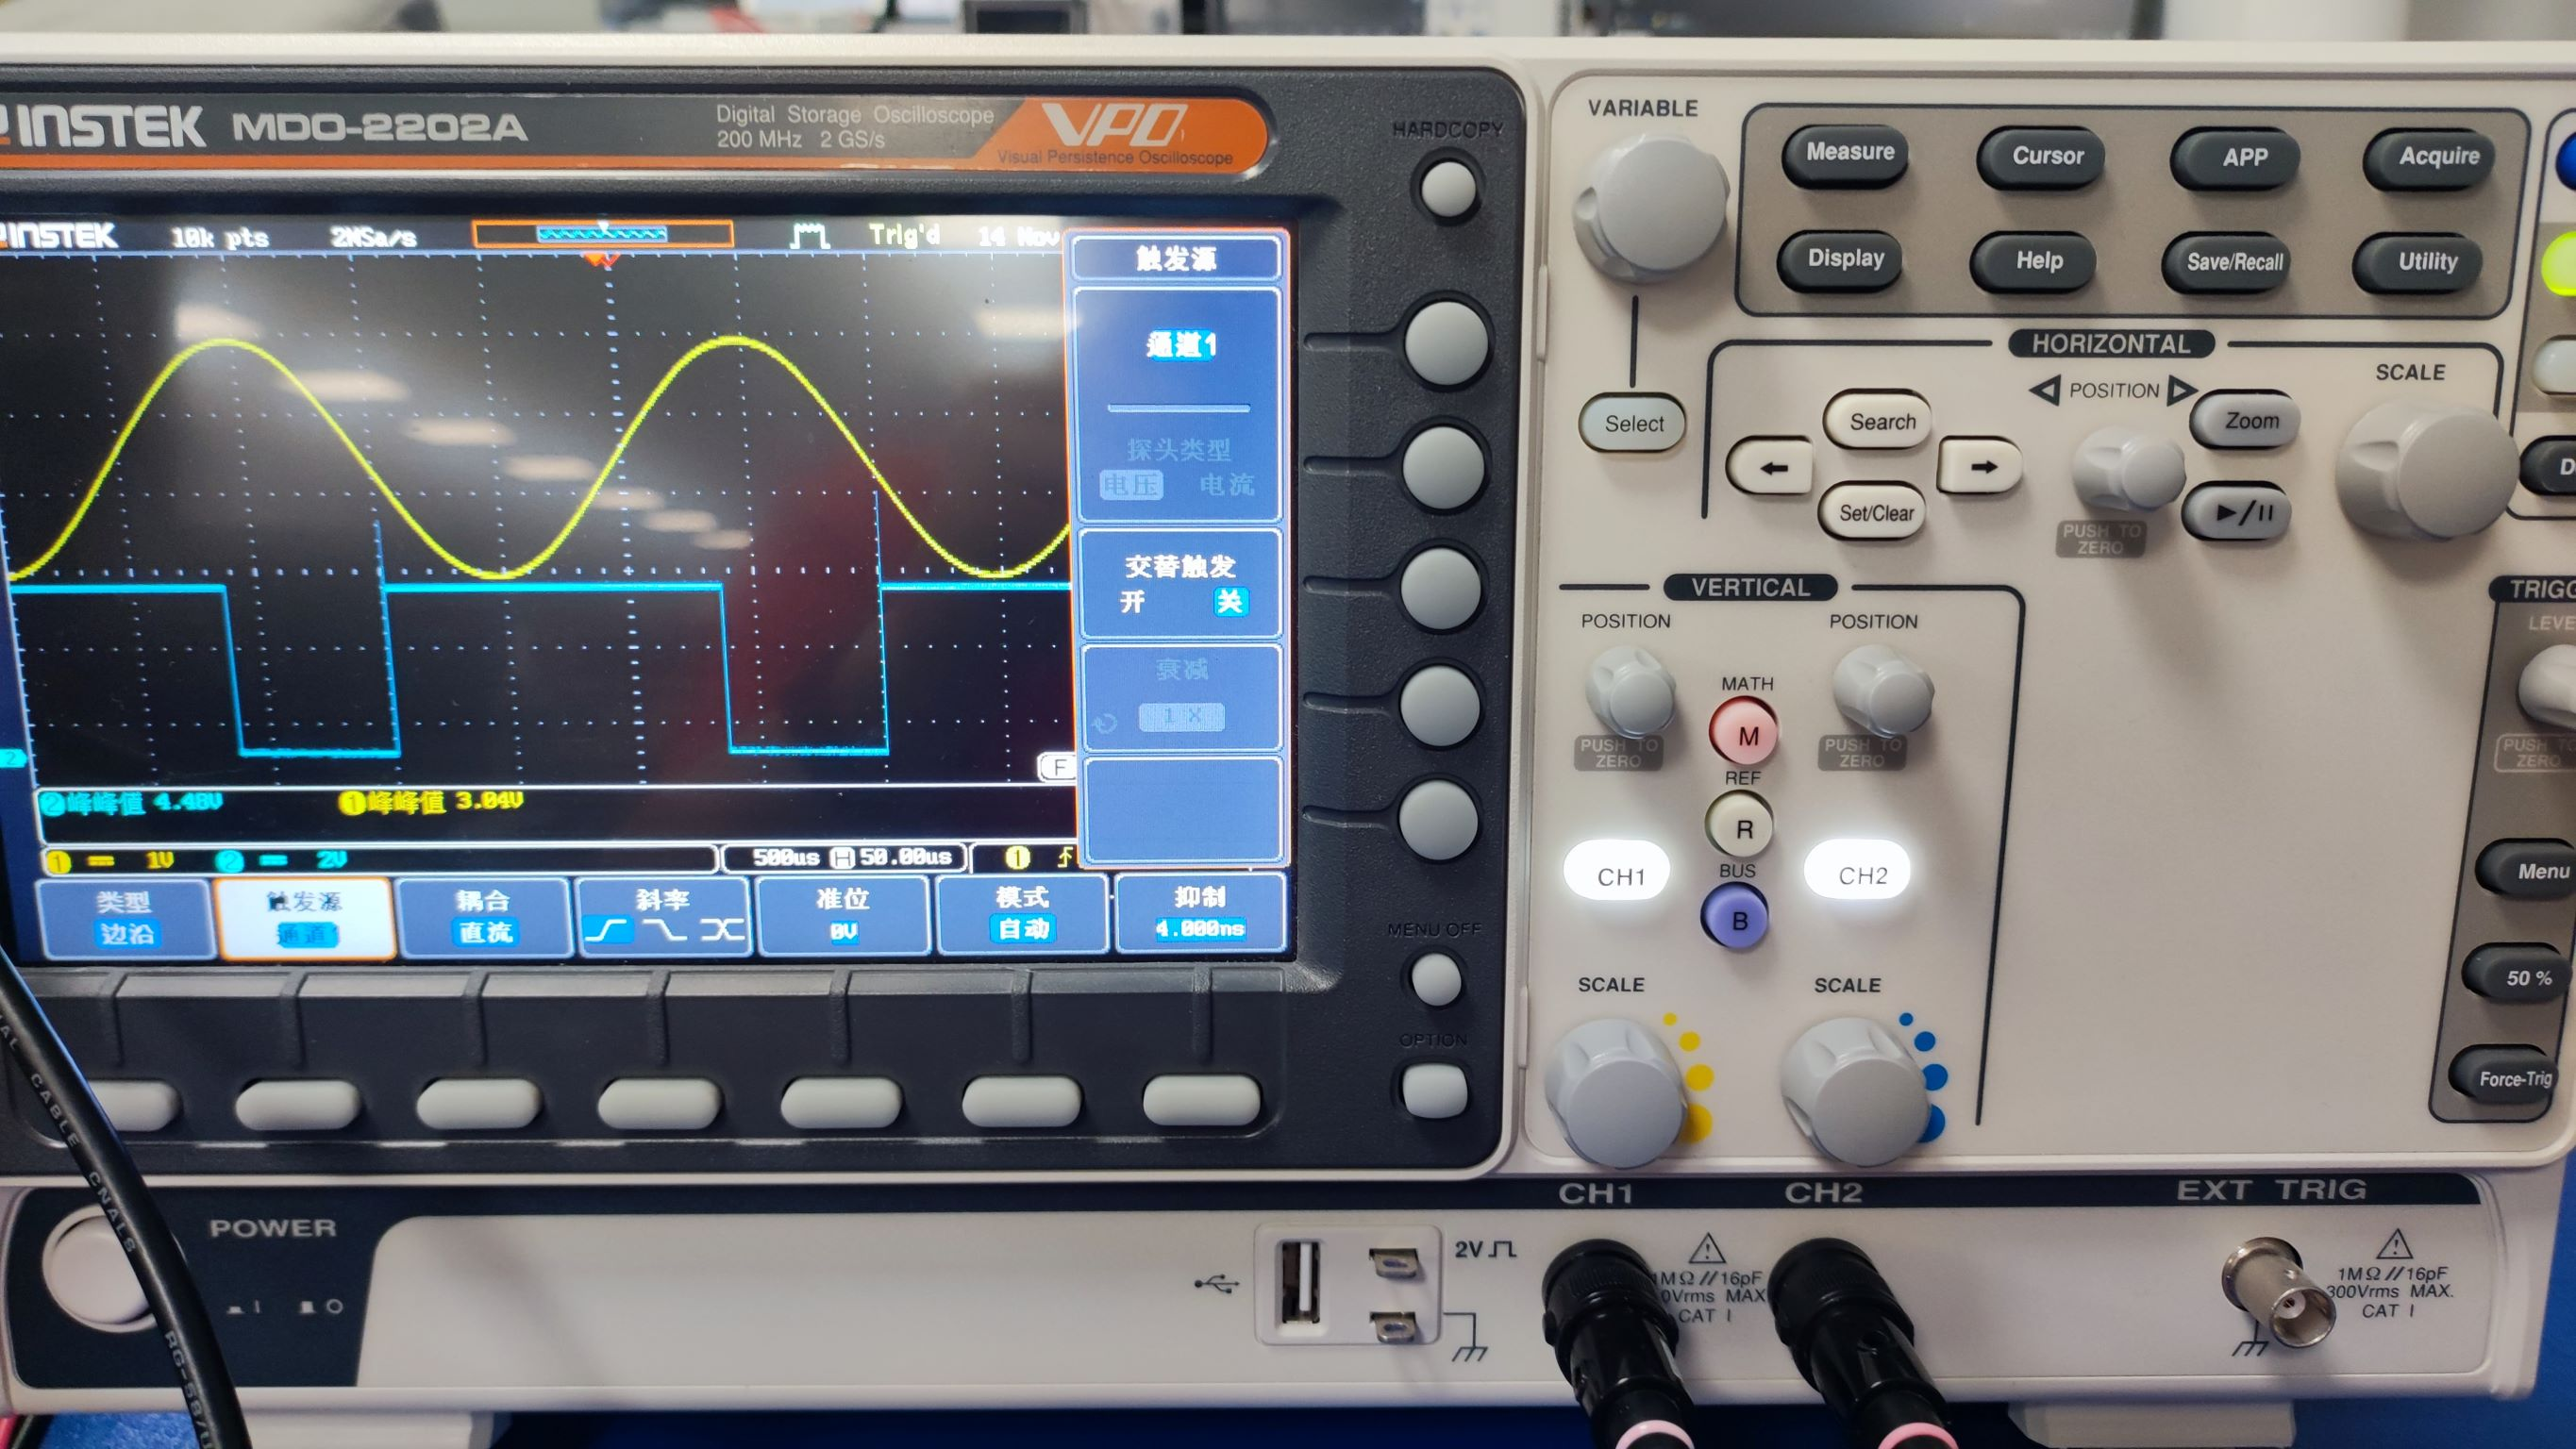
\includegraphics[width=0.9\linewidth]{../图片/555示波器2}
			\caption{555示波器2}
		\end{minipage}
		\begin{minipage}[t]{0.5\linewidth}
			\centering
			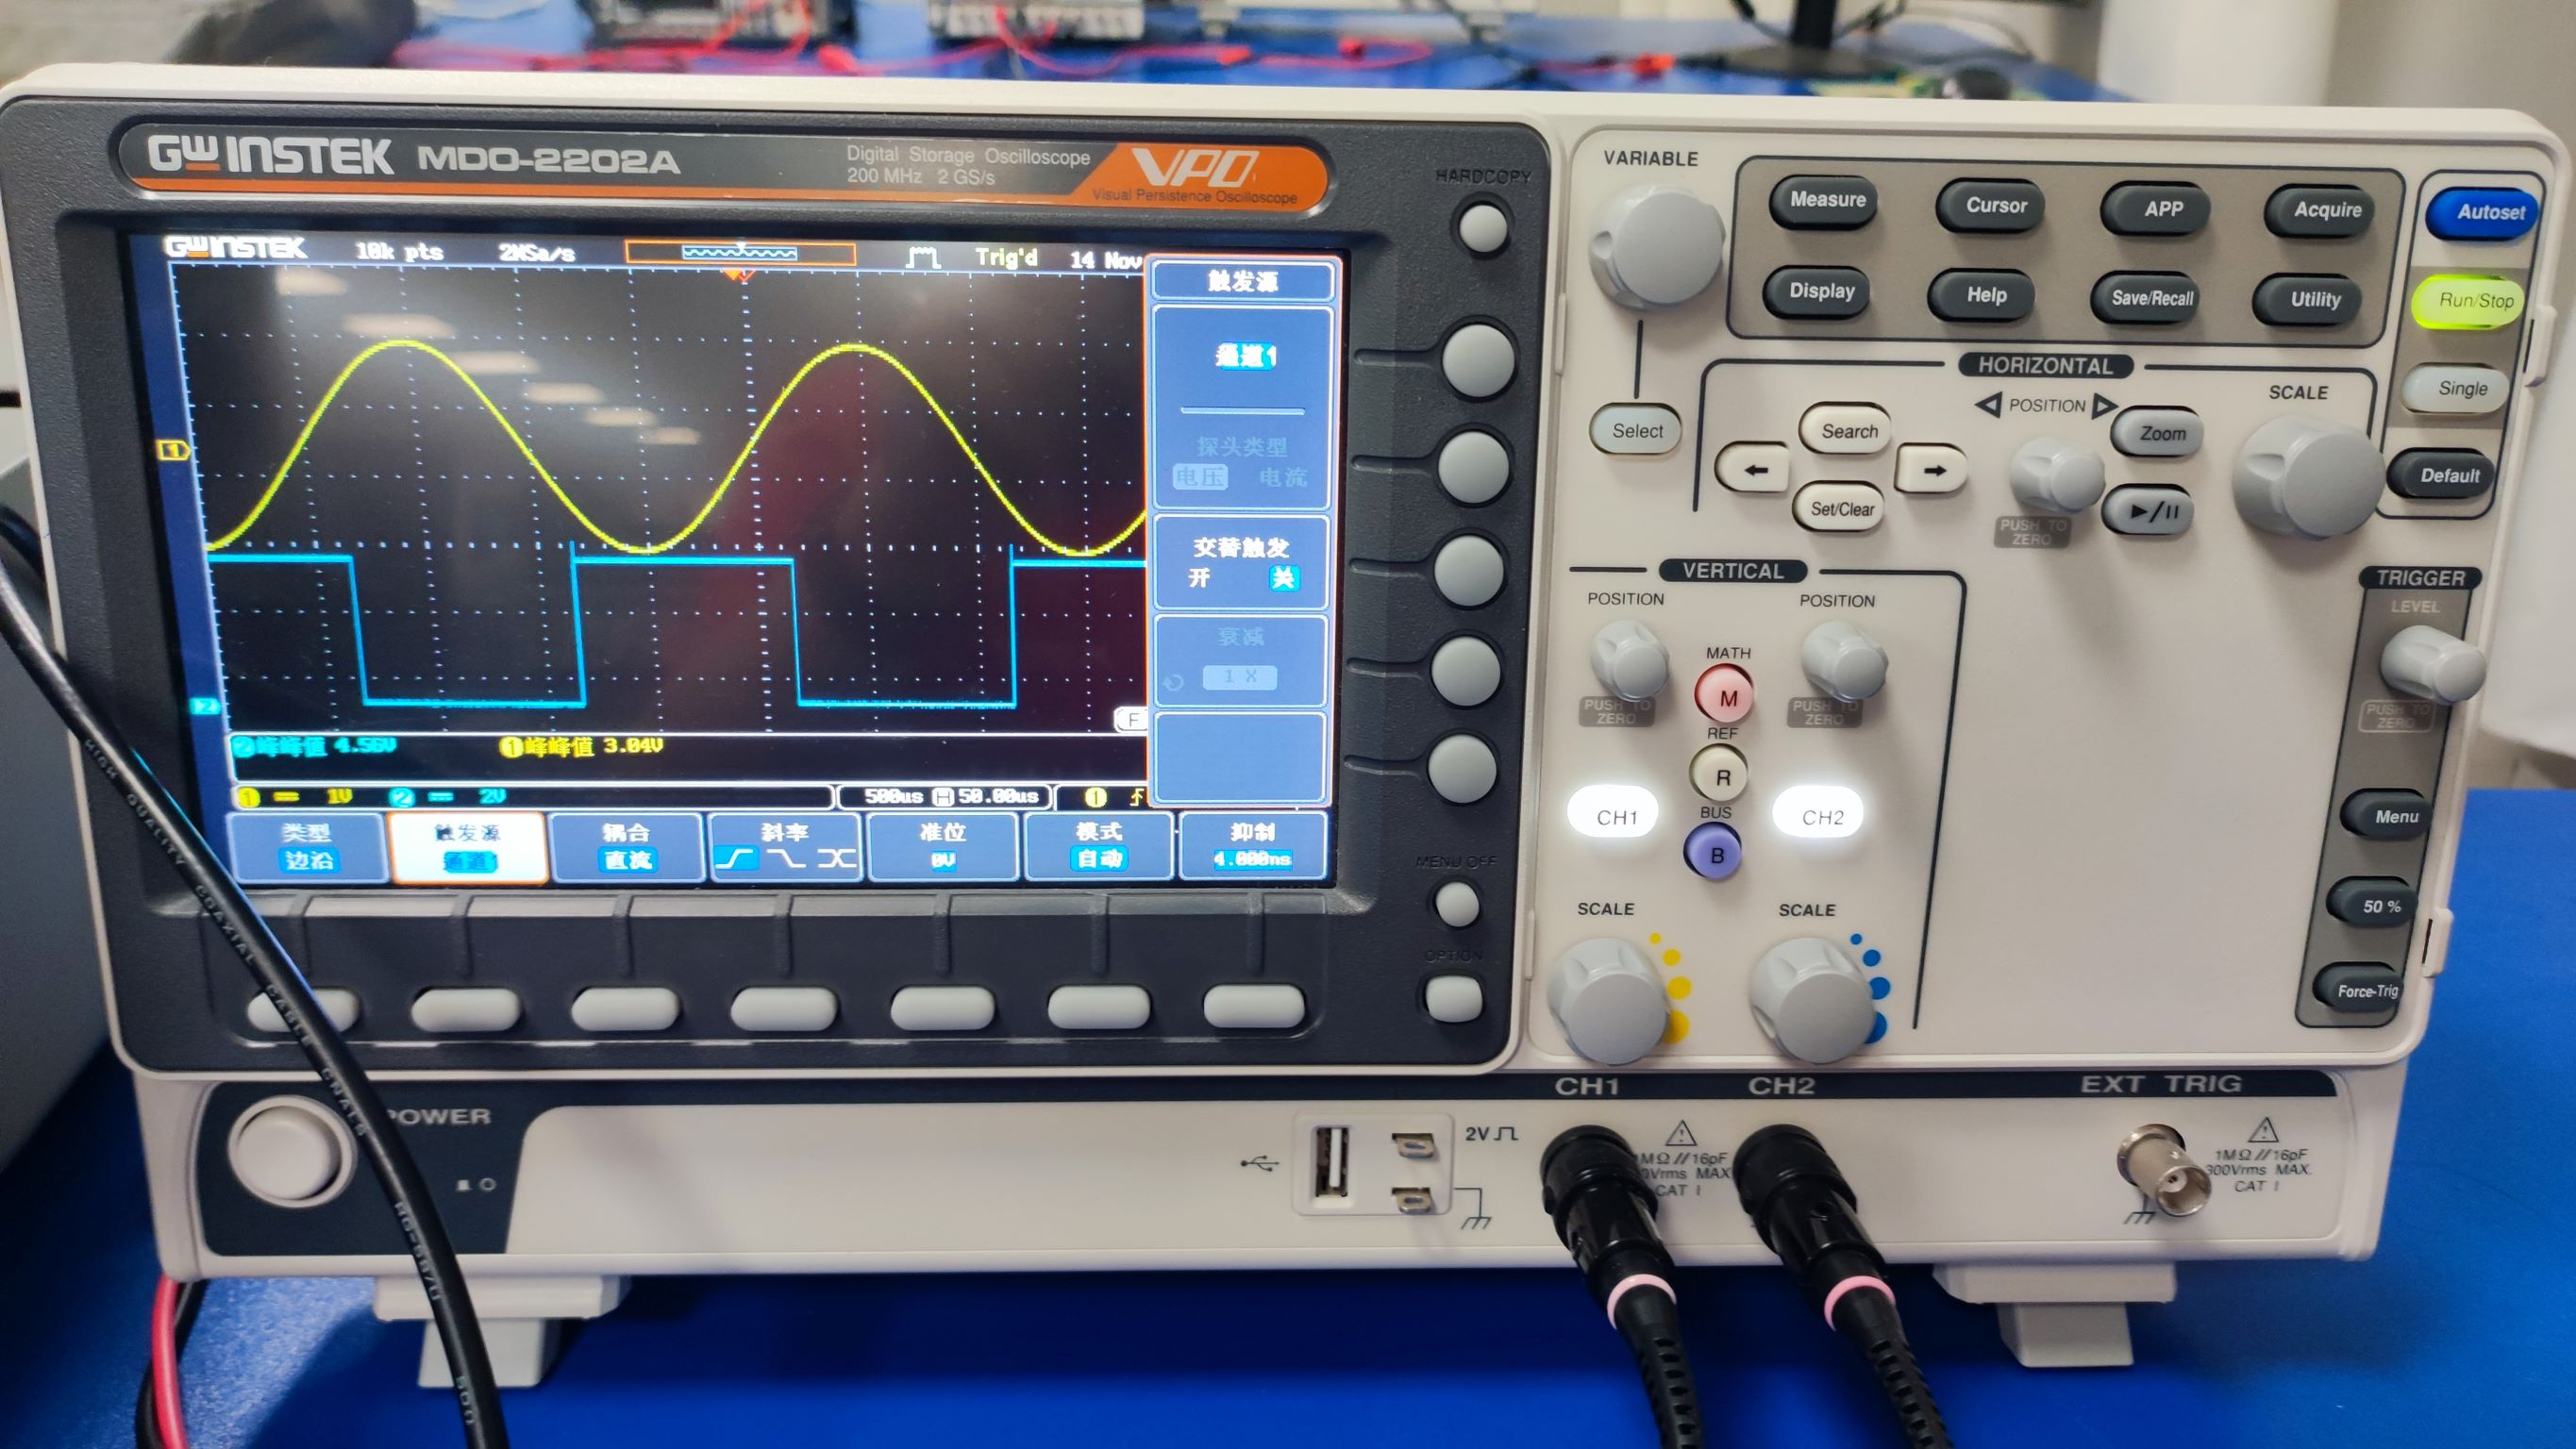
\includegraphics[width=0.9\linewidth]{../图片/555示波器3}
			\caption{555示波器3}
		\end{minipage}
	\end{figure}

\end{document}